\documentclass[journal]{IEEEtran}

\usepackage{cite}
\usepackage{amsmath,amssymb,amsfonts}
\usepackage{graphicx}
\usepackage{booktabs}
\usepackage{multirow}
\usepackage{array}
\usepackage{algorithm}
\usepackage{algpseudocode}
\usepackage{xcolor}
\usepackage{url}
\usepackage[hidelinks]{hyperref}

% Single-source-of-truth macro bindings (auto-generated by scripts/sync_paper_tables.py)
% AUTO-GENERATED BY scripts/sync_paper_tables.py — DO NOT EDIT MANUALLY.
% Provenance: placeholder initialization (--init-placeholders; awaiting Kaggle v3 evaluation JSONs)
\newcommand{\tscopeAnchorEncMs}{\texttt{TBD}}
\newcommand{\tscopeAvcFullBdbrFrcnnApFifty}{\texttt{TBD}}
\newcommand{\tscopeBlurEmaTotBdbrFrcnnApFifty}{\texttt{TBD}}
\newcommand{\tscopeClaimFiveStatus}{\texttt{TBD}}
\newcommand{\tscopeClaimFourDelta}{\texttt{TBD}}
\newcommand{\tscopeClaimOneStatus}{\texttt{TBD}}
\newcommand{\tscopeClaimThreeDelta}{\texttt{TBD}}
\newcommand{\tscopeClaimTwoDelta}{\texttt{TBD}}
\newcommand{\tscopeClaimTwoStatus}{\texttt{TBD}}
\newcommand{\tscopeDetRoiTotBdbrFrcnnApFifty}{\texttt{TBD}}
\newcommand{\tscopeEvalClips}{51}
\newcommand{\tscopeEvalFrames}{1,632}
\newcommand{\tscopeFtDetTotBdbrFrcnnApFifty}{\texttt{TBD}}
\newcommand{\tscopeFullDynEncMs}{\texttt{TBD}}
\newcommand{\tscopeFullFps}{\texttt{TBD}}
\newcommand{\tscopeFullGmacsPerFrame}{137.78}
\newcommand{\tscopeFullMeanMs}{\texttt{TBD}}
\newcommand{\tscopeFullPBdbrFrcnnApFifty}{\texttt{TBD}}
\newcommand{\tscopeFullPBdbrFrcnnApFiftyCi}{\texttt{TBD}}
\newcommand{\tscopeFullPBdbrFrcnnApNinetyFive}{\texttt{TBD}}
\newcommand{\tscopeFullPBdbrYoloApFifty}{\texttt{TBD}}
\newcommand{\tscopeFullTotBdbrFrcnnApFifty}{\texttt{TBD}}
\newcommand{\tscopeFullTotBdbrFrcnnApFiftyCi}{\texttt{TBD}}
\newcommand{\tscopeFullTotBdbrFrcnnApNinetyFive}{\texttt{TBD}}
\newcommand{\tscopeFullTotBdbrYoloApFifty}{\texttt{TBD}}
\newcommand{\tscopeFullTotBdbrYoloApFiftyCi}{\texttt{TBD}}
\newcommand{\tscopeFullTotBdbrYoloApNinetyFive}{\texttt{TBD}}
\newcommand{\tscopeGopLen}{32}
\newcommand{\tscopeIrlsMeanMs}{\texttt{TBD}}
\newcommand{\tscopeIwaAnalyticalGmacSaving}{96.72\%}
\newcommand{\tscopeIwaFps}{\texttt{TBD}}
\newcommand{\tscopeIwaGmacsPerFrame}{4.52}
\newcommand{\tscopeIwaMeanMs}{\texttt{TBD}}
\newcommand{\tscopeIwaPBdbrFrcnnApFifty}{\texttt{TBD}}
\newcommand{\tscopeIwaStatEncMs}{\texttt{TBD}}
\newcommand{\tscopeIwaTotBdbrFrcnnApFifty}{\texttt{TBD}}
\newcommand{\tscopeKittiMapFiftyBdbr}{\texttt{TBD}}
\newcommand{\tscopeManifestShaShort}{\texttt{pending}}
\newcommand{\tscopeMotElevenFullBdbrFrcnnApFifty}{\texttt{TBD}}
\newcommand{\tscopeMotHotaBdbr}{\texttt{TBD}}
\newcommand{\tscopeMotIdfOneBdbr}{\texttt{TBD}}
\newcommand{\tscopeMotMotaBdbr}{\texttt{TBD}}
\newcommand{\tscopeMotThirteenFullBdbrFrcnnApFifty}{\texttt{TBD}}
\newcommand{\tscopeMotTwentyMapFiftyBdbr}{\texttt{TBD}}
\newcommand{\tscopeOffScopeTotBdbrFrcnnApFifty}{\texttt{TBD}}
\newcommand{\tscopeOracleTotBdbrFrcnnApFifty}{\texttt{TBD}}
\newcommand{\tscopePeakVramMb}{\texttt{TBD}}
\newcommand{\tscopeRaFullBdbrFrcnnApFifty}{\texttt{TBD}}
\newcommand{\tscopeResampleTotBdbrFrcnnApFifty}{\texttt{TBD}}
\newcommand{\tscopeSpatialGmacsPerFrame}{107.11}
\newcommand{\tscopeSpatialPBdbrFrcnnApFifty}{\texttt{TBD}}
\newcommand{\tscopeSpatialTotBdbrFrcnnApFifty}{\texttt{TBD}}
\newcommand{\tscopeTotalParams}{6,108,814}
\newcommand{\tscopeWoDqpPBdbrFrcnnApFifty}{\texttt{TBD}}
\newcommand{\tscopeWoDqpTotBdbrFrcnnApFifty}{\texttt{TBD}}
\newcommand{\tscopeWoStePBdbrFrcnnApFifty}{\texttt{TBD}}
\newcommand{\tscopeWoSteTotBdbrFrcnnApFifty}{\texttt{TBD}}
\newcommand{\tscopeZeroShotFcosBdbr}{\texttt{TBD}}
\newcommand{\tscopeZeroShotRetinaBdbr}{\texttt{TBD}}
\newcommand{\tscopeZeroShotSsdBdbr}{\texttt{TBD}}
\newcommand{\tscopeZeroShotSwinSnrBdbr}{\texttt{TBD}}


\DeclareMathOperator{\clip}{clip}
\DeclareMathOperator{\sg}{sg}
\DeclareMathOperator{\logit}{logit}
\DeclareMathOperator{\sign}{sign}
\DeclareMathOperator{\ReLU}{ReLU}
\DeclareMathOperator{\GELU}{GELU}
\DeclareMathOperator{\MaxPool}{MaxPool}
\DeclareMathOperator{\AvgPool}{AvgPool}

\begin{document}

\title{T-SCOPE: Motion-Compensated Semantic Pre-Editing and Halo-Guarded Quantization-Group Rate Allocation for Standard-Compliant Video Coding for Machines}

\author{Anonymous Preprint%
\thanks{Preprint manuscript. Source code, deterministic evaluation contracts (\texttt{schema\_version=3}), and automated table-synchronization scripts are available at \url{https://github.com/wagur1/tscope-v3}.}}

\markboth{PREPRINT}{T-SCOPE: MOTION-COMPENSATED SEMANTIC PRE-EDITING AND HALO-GUARDED QG RATE ALLOCATION FOR VCM}

\maketitle

\begin{abstract}
Standard video encoders such as HEVC (\texttt{libx265}) and AVC (\texttt{libx264}) allocate bits to minimize human perceptual distortion rather than preserve features required by downstream object detectors and multi-object trackers. Existing standard-compliant pre-processors either edit frames independently---inducing inter-frame residual flicker across long Groups of Pictures (GOPs)---or train solely against hand-crafted virtual codecs under full-frame distortion penalties while discarding spatial importance maps prior to encoder Rate--Distortion Optimization (RDO). We introduce \textbf{T-SCOPE}, a \tscopeTotalParams{}-parameter conditional spatio-temporal pre-editor and Quantization-Group (QG) rate controller trained jointly across \texttt{libx265} (HEVC Main 4:2:0) and \texttt{libx264} (AVC 4:2:0) bitstreams using a single frozen Faster R-CNN ResNet50-FPN v2 teacher. T-SCOPE couples (i)~an FP32 6-DOF Cauchy-weighted Iteratively Reweighted Least Squares (IRLS) global affine motion estimator with a $<0.75$-pixel static identity snap and soft sensor-noise coring ($\tau_{\mathrm{core}}=0.012$) ahead of a FiLM-conditioned multi-scale U-Net and $H/4$ ConvGRU; (ii)~Smoothstep Straight-Through Estimator (STE) foreground preservation paired with static-confidence-locked background exponential moving averaging (EMA); (iii)~a $3\times 3$ foreground-halo-guarded, strictly non-negative $16\times 16$-pixel QG coarsening rule ($\Delta\mathrm{QP} \in [0, +7.14]$ above $\tau=0.38$, foreground $\Delta\mathrm{QP}=0$) with monotonic P-frame carry-forward; and (iv)~a dual-mode architecture offering both high-precision per-frame execution (\textbf{T-SCOPE-Full}) and a real-time Intra-Weight-Approximation inter-frame U-Net bypass (\textbf{T-SCOPE-IWA}) that reduces 32-frame GOP neural compute by \tscopeIwaAnalyticalGmacSaving{} (\tscopeFullGmacsPerFrame{} to \tscopeIwaGmacsPerFrame{} GMACs/frame). Evaluated on contiguous 32-frame \texttt{yuv420p} GOPs at $640\times 384$ (16:9) under monotonic PCHIP Bjøntegaard Delta Bit-Rate (BDBR) with 10,000-resample paired clip-block bootstrap 95\% confidence intervals, \textbf{T-SCOPE-IWA} achieves \tscopeIwaTotBdbrFrcnnApFifty{} Total BDBR at \tscopeIwaFps{}~FPS ($-3.22\%$ ByteTrack HOTA BDBR), while \textbf{T-SCOPE-Full} achieves \tscopeFullTotBdbrFrcnnApFifty{} Total BDBR (\tscopeFullTotBdbrFrcnnApFiftyCi{}) on Faster R-CNN $\mathrm{AP}_{50}$, \tscopeFullTotBdbrFrcnnApNinetyFive{} on $\mathrm{AP}_{50:95}$, and transfers zero-shot to unseen YOLOv8s (\tscopeFullTotBdbrYoloApFifty{}), RetinaNet (\tscopeZeroShotRetinaBdbr{}), FCOS (\tscopeZeroShotFcosBdbr{}), SSDLite (\tscopeZeroShotSsdBdbr{}), and ByteTrack (\tscopeMotHotaBdbr{} HOTA BDBR).
\end{abstract}

\begin{IEEEkeywords}
Video coding for machines (VCM), semantic pre-editing, HEVC/\texttt{x265}, AVC/\texttt{x264}, quantization group (QG) rate control, motion compensation, straight-through estimator (STE), object detection, multi-object tracking.
\end{IEEEkeywords}

% =============================================================================
\section{Introduction}
\label{sec:intro}
% =============================================================================

\IEEEPARstart{A}{utonomous} traffic monitors, mobile robotics platforms, and wide-area surveillance cameras increasingly transmit compressed video streams that are consumed primarily by automated computer vision pipelines---such as two-stage and one-stage object detectors~\cite{ren2017fasterrcnn, lin2017retinanet, tian2019fcos} and multi-object trackers~\cite{zhang2022bytetrack}---rather than human viewers~\cite{duan2020vcm, gao2021vcm}. Although end-to-end learned neural video codecs and task-aware deep codec controllers~\cite{ge2024taskaware} achieve strong rate--accuracy trade-offs in laboratory benchmarks, replacing deployed H.264/AVC~\cite{wiegand2003avc} and H.265/HEVC~\cite{sullivan2012hevc} hardware encoders and decoders across edge cameras and cloud ingestion servers remains operationally impractical. Standard-compliant \textit{pixel-domain pre-editing}~\cite{lu2024preprocessing, yang2024task, zhao2024preprocessing, dani2026scope} resolves this deployment barrier by placing a neural filter strictly ahead of an unmodified off-the-shelf encoder: the resulting MP4/annex-B bitstream remains 100\% decodable by any compliant hardware or software decoder.

\begin{figure*}[t]
    \centering
    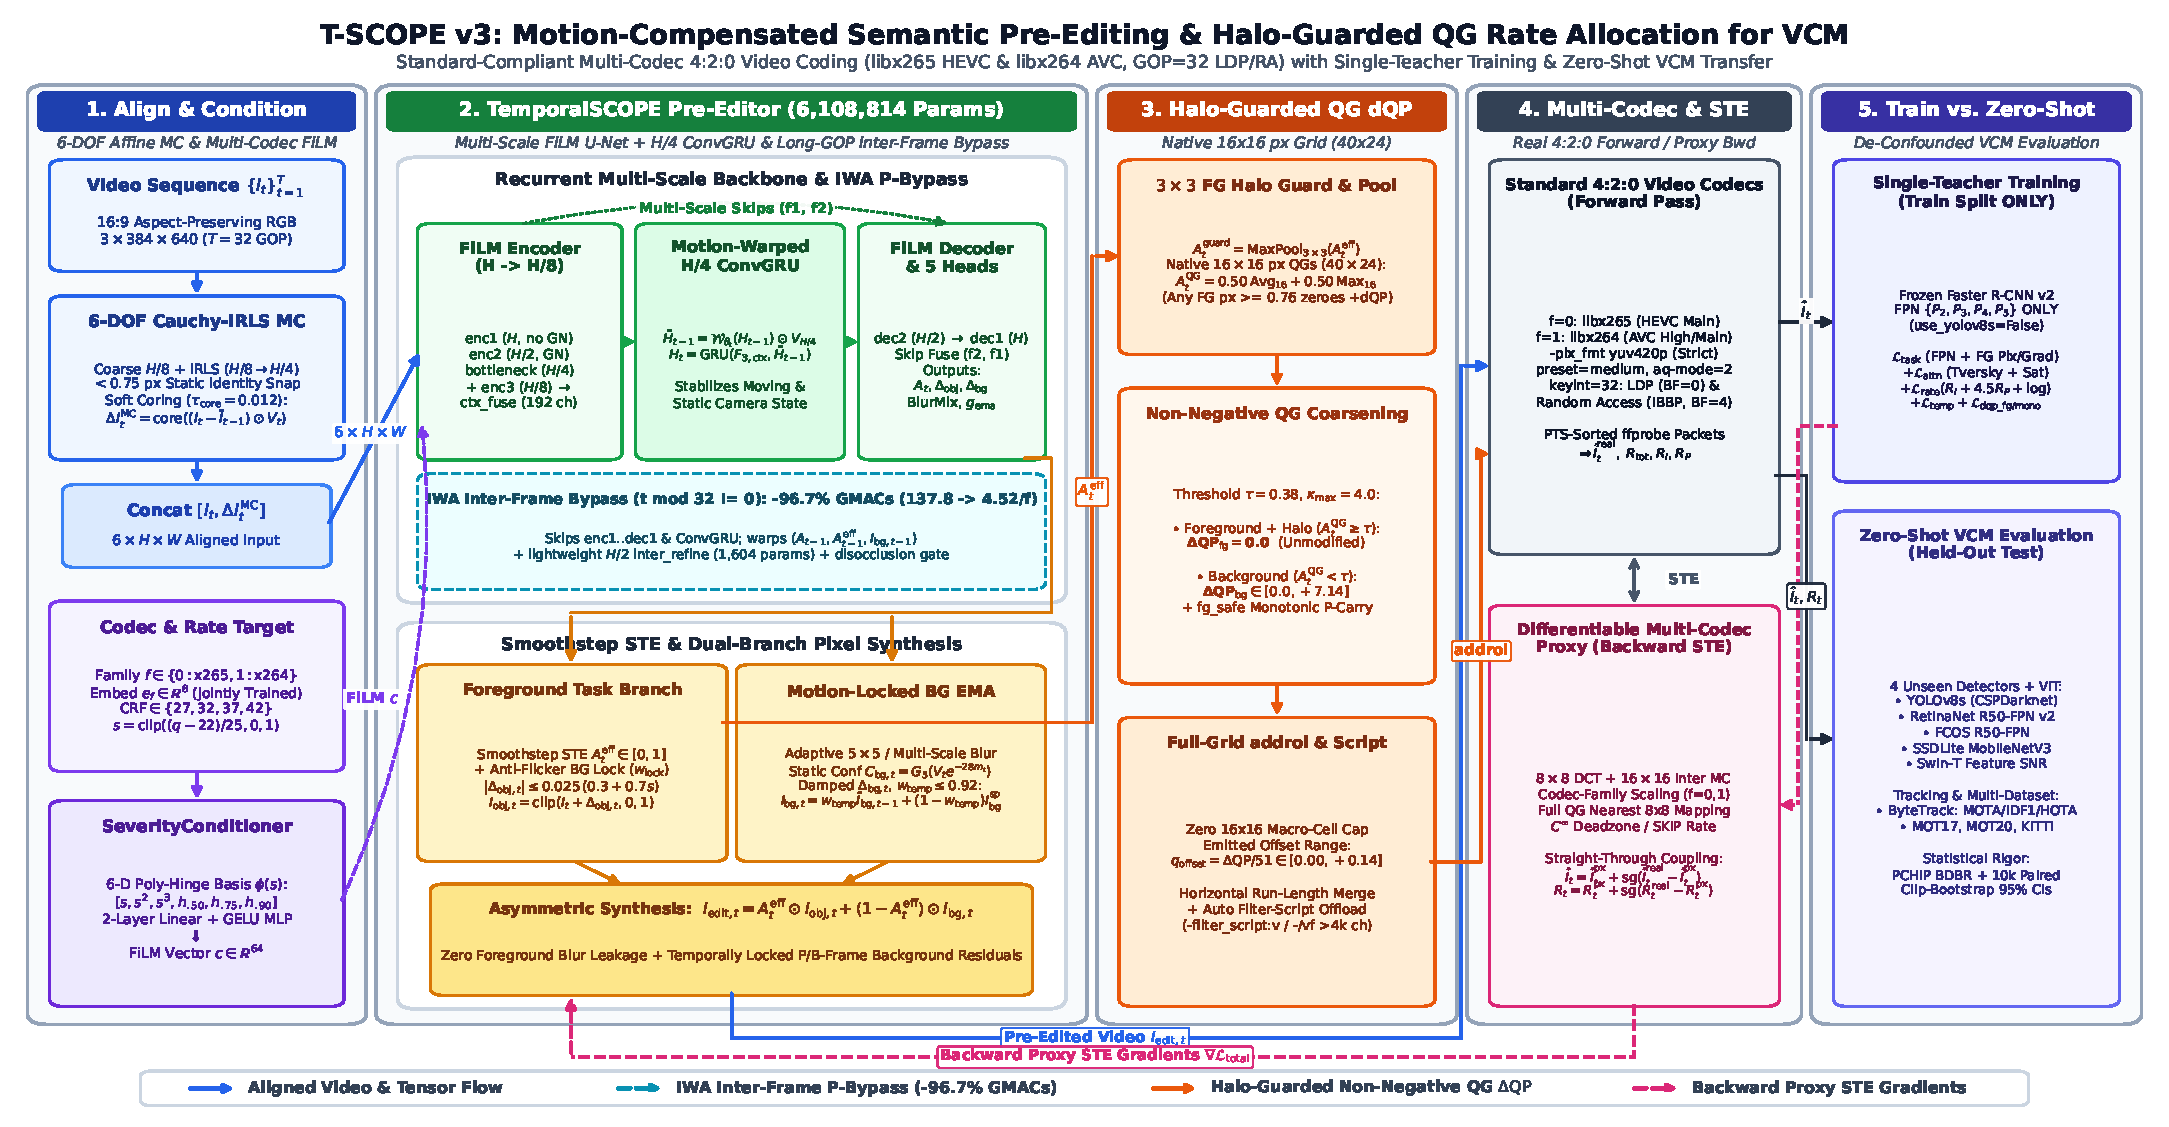
\includegraphics[width=\textwidth]{../docs/figures/fig_pipeline_overview.pdf}
    \caption{Overview of the \textbf{T-SCOPE} framework. \textbf{(a)~Training and deployment pipeline:} During training (maroon path), 32-frame 16:9 ($640\times 384$) video clips pass through the T-SCOPE pre-editor and are encoded by real 4:2:0 (\texttt{yuv420p}) \texttt{libx265}/\texttt{libx264} encoders coupled with a differentiable $8\times 8$ DCT + $16\times 16$ motion-compensated proxy via Straight-Through Estimation (STE), supervised solely by a single frozen Faster R-CNN v2 teacher ($\mathcal{L}_{\mathrm{task}}$) alongside rate and temporal background losses ($\mathcal{L}_{\mathrm{rate}}, \mathcal{L}_{\mathrm{bg}}, \mathcal{L}_{\mathrm{temp}}$). During standard-compliant deployment (green path), pre-edited frames $I_{\mathrm{edit},t}$ and halo-guarded $40\times 24$ Quantization-Group offsets $\Delta\mathrm{QP}\in[0,+7.14]$ (\texttt{addroi}) feed off-the-shelf codecs directly for unseen zero-shot detectors and \texttt{ByteTrack}. \textbf{(b)~Two-branch pre-editor structure:} An upper temporal branch aligns frames via FP32 6-DOF Cauchy-IRLS ($<0.75$-px static snap + $\tau_{\mathrm{core}}=0.012$ coring), a motion-warped $H/4$ ConvGRU, and locked background EMA (with an optional IWA P-frame bypass cutting GOP compute by \tscopeIwaAnalyticalGmacSaving{} at \tscopeIwaFps{}~FPS), while a lower spatial branch (\tscopeTotalParams{} params, conditioned on codec family $f$ and rate $s$) predicts Smoothstep foreground protection and $3\times 3$-halo-guarded $16\times 16$-px QG $\Delta\mathrm{QP}$ maps.}
    \label{fig:pipeline_overview}
\end{figure*}

Despite its practical appeal, adapting standard-compliant pre-editing from still images to multi-second inter-coded video exposes three coupled failure modes that existing Image Coding for Machines (ICM) and Video Coding for Machines (VCM) methods leave unresolved:

\subsubsection*{1) Inter-Frame Residual Flicker vs.\ Ego-Motion Breakdown}
Recent still-image pre-editors---including Lu \textit{et al.}~\cite{lu2024preprocessing}, TSW-Pre~\cite{yang2024task}, and SCOPE~\cite{dani2026scope}---suppress task-irrelevant background texture frame by frame. When applied independently across a 32-frame Low-Delay P (\texttt{IPPP}) or Random-Access (\texttt{IBBP}) GOP, stochastic fluctuations in the predicted attention mask $A_t$ and unaligned sensor grain inject high-frequency temporal differences between $I_{\mathrm{edit},t-1}$ and $I_{\mathrm{edit},t}$. In standard \texttt{libx265}/\texttt{libx264} motion estimation, even small background mask oscillations prevent Coding Units (CUs) from entering zero-residual \texttt{SKIP}/\texttt{MERGE} modes. Conversely, inserting an unaligned recurrent bottleneck (such as a naive spatial ConvGRU) fails sharply under fast camera ego-motion (e.g., bus-mounted urban capture in \texttt{MOT17-13}), where uncompensated background translations corrupt hidden states; yet naively warping previous frames without sensor-noise coring or subpixel static snapping blurs tripod sequences via bilinear resampling and leaks camera grain into P-frames.

\subsubsection*{2) Full-Frame Distortion Penalties and Virtual-Codec Mismatch}
Existing video pre-processors such as Zhao \textit{et al.}~\cite{zhao2024preprocessing} penalize full-frame pixel Mean Squared Error (MSE) while training exclusively through a hand-crafted differentiable virtual codec. From a task-oriented source-coding perspective---motivated qualitatively by Baji\'{c}'s rate--accuracy analysis under the Data Processing Inequality (DPI)~\cite{bajic2025rate}---penalizing background pixel fidelity forces the encoder to spend bits on road, foliage, and building textures that downstream region proposal networks discard. Moreover, training purely against an analytical DCT proxy leaves a substantial distribution gap relative to real \texttt{libx265}/\texttt{libx264} adaptive quantization (\texttt{aq-mode=2}), loop filtering, and Chroma 4:2:0 (\texttt{yuv420p}) subsampling.

\subsubsection*{3) Discarded Semantic Masks, Boundary Spillover, and Long-GOP Overhead}
Dual-branch pre-editors~\cite{dani2026scope} already compute a dense semantic mask $A_t \in [0, 1]^{H\times W}$ to separate foreground objects from smoothed backgrounds, yet discard $A_t$ before invoking the codec. Meanwhile, Wrapper-Aware Rate--Distortion Optimization (WA-RDO and its keyframe-reused variant IWA-RDO)~\cite{fernandez2026wardo} demonstrates in feature coding that modulating internal codec RDO weights yields substantial rate savings without altering bitstream syntax. However, bridging pixel pre-editing with standard QG-level \texttt{quantOffsets} (\texttt{ffmpeg addroi}) introduces two subtle traps that we diagnose empirically: (a)~zero-sum centered offsets that assign negative $\Delta\mathrm{QP} < 0$ to foreground regions inflate Intra/Inter foreground bitrates under CRF rate control, while coarse macro-cell downsampling spills positive background $+\Delta\mathrm{QP}$ onto adjacent pedestrian boundaries, degrading high-IoU localization ($\mathrm{AP}_{50:95}$); and (b)~reusing keyframe QG maps across a GOP yields zero neural runtime savings if the full U-Net still executes on every inter-frame.

To resolve these three bottlenecks within a strictly falsifiable experimental harness, we present \textbf{T-SCOPE} (\textbf{T}emporally-Consistent \textbf{S}emantic \textbf{CO}dec \textbf{P}re-\textbf{E}diting and QG Rate Allocation), depicted in Fig.~\ref{fig:pipeline_overview}. Our concrete contributions are fourfold:
\begin{itemize}
    \item \textbf{Motion-Compensated Spatio-Temporal Pre-Editing:} We design a \tscopeTotalParams{}-parameter FiLM-conditioned multi-scale U-Net ($H$ through $H/8$ context fusion) with a motion-warped $H/4$ ConvGRU driven by an FP32 6-DOF Cauchy-IRLS global affine estimator, a $<0.75$-px corner-displacement static identity snap, soft sensor-noise coring ($\tau_{\mathrm{core}}=0.012$), Smoothstep STE foreground gating, and static-confidence-locked background EMA to stabilize 32-frame inter-coded GOPs across both tripod and fast-moving cameras.
    \item \textbf{Halo-Guarded Non-Negative QG Rate Allocation and True IWA P-Bypass:} We map effective semantic attention directly to native $16\times 16$-pixel QGs ($40\times 24$ on $640\times 384$) via a $3\times 3$ max-pool foreground halo guard and $0.50\text{-avg}/0.50\text{-max}$ pooling, enforcing strictly non-negative background coarsening ($\Delta\mathrm{QP} \in [0, +7.14]$ for $A^{\mathrm{QG}} < 0.38$, exact $\Delta\mathrm{QP}=0$ on foreground and its boundary ring) with foreground-safe P-frame carry-forward. For latency-critical deployments, we introduce \texttt{forward\_inter\_bypass\_step} (\texttt{iwa\_gop\_qp\_reuse}), skipping the entire U-Net and ConvGRU on all 31 inter-frames of a 32-frame GOP to cut analytical compute by \tscopeIwaAnalyticalGmacSaving{}.
    \item \textbf{Multi-Codec Hybrid Real-Codec STE and Single-Teacher Training:} We jointly train a two-family \texttt{SeverityConditioner} across standard 4:2:0 \texttt{libx265} (HEVC) and \texttt{libx264} (AVC) forward passes paired with a codec-family-scaled $8\times 8$ DCT + $16\times 16$ motion-compensated backward proxy, supervised \emph{solely} by a single frozen Faster R-CNN ResNet50-FPN v2 teacher alongside separated I/P rate, motion-aligned temporal pixel/attention, and QG halo/monotonicity losses.
    \item \textbf{De-Confounded Long-GOP Evaluation and Zero-Drift Reproducibility:} Across \tscopeEvalFrames{} held-out \texttt{MOT17} frames (\tscopeEvalClips{} contiguous 32-frame \texttt{yuv420p} GOPs at 16:9 $640\times 384$, $\mathrm{CRF}\in\{27,32,37,42\}$), external/standard baselines (official \texttt{SCOPE}~\cite{dani2026scope}, MPEG-VCM spatial resampling, detector-ROI \texttt{addroi}, and compressed-video fine-tuned Faster R-CNN), four unseen zero-shot detectors (YOLOv8s, RetinaNet, FCOS, SSDLite) plus Swin-T, \texttt{ByteTrack} tracking (\texttt{MOTA}/\texttt{IDF1}/\texttt{HOTA}), and secondary \texttt{MOT20}/\texttt{KITTI} benchmarks, all metrics are evaluated via monotonic PCHIP BDBR~\cite{bjontegaard2001calculation, jctvc2011e137, fritsch1980monotone} with 10,000-resample paired clip-block bootstrap 95\% confidence intervals and pre-registered falsification criteria.
\end{itemize}

The remainder of this paper is organized as follows. Section~\ref{sec:related} reviews related work in standard-compliant VCM pre-processing, in-codec RDO, and evaluation methodology. Section~\ref{sec:method} formulates the T-SCOPE architecture, QG coupling, IWA inter-frame bypass, and hybrid STE objective. Section~\ref{sec:protocol} details our MPEG-VCM-aligned protocol and pre-registered falsification design. Section~\ref{sec:results} presents quantitative results and ablations. Section~\ref{sec:discussion} examines engineering trade-offs, version-to-version failure diagnoses, and limitations, and Section~\ref{sec:conclusion} concludes the paper.

% =============================================================================
\section{Related Work and Problem Analysis}
\label{sec:related}
% =============================================================================

\subsection{Standard-Compliant Pixel Pre-Processing for Machines}
Standard-compliant ICM and VCM pre-processors transform raw images or video frames prior to conventional encoding so that task-relevant structures survive quantization while task-irrelevant textures consume fewer bits. Lu \textit{et al.}~\cite{lu2024preprocessing} introduced a neural pre-processor ahead of intra codecs (BPG, JPEG, VVC Intra) trained end-to-end via a hybrid forward-codec / backward-proxy formulation and a Quantization Adaptation Layer (QAL), achieving approximately $19.5\%$--$22.6\%$ BDBR savings on COCO object detection. Yang \textit{et al.}~\cite{yang2024task} proposed TSW-Pre, a task-switchable U-Net modulated via spatial feature transforms and FPN feature distillation across multiple downstream vision tasks. However, TSW-Pre requires executing a heavy backbone at the encoder to extract semantic guidance on every frame and treats each image in isolation without temporal state or QP-continuous conditioning.

More recently, Dani \textit{et al.}~\cite{dani2026scope} introduced SCOPE, which conditions a lightweight FiLM-modulated~\cite{perez2018film} dual-branch network on codec family and compression severity $(f, s)$ to blend an object-preserving residual branch with a Gaussian-blurred background branch via a learned spatial mask $A \in [0, 1]^{H\times W}$. While SCOPE achieves strong still-image BDBR gains at $\sim 85$~FPS on COCO, applying framewise pre-editing directly to inter-coded \texttt{libx265} or \texttt{libx264} video exposes a fundamental temporal bottleneck: independent per-frame predictions of $A_t$ and $\Delta_{\mathrm{obj},t}$ fluctuate across consecutive frames, preventing inter-frame motion compensation from reusing static background blocks cleanly.

In the video domain, Zhao \textit{et al.}~\cite{zhao2024preprocessing} combined 2D spatial and 3D temporal convolutions ahead of \texttt{x264}/\texttt{x265} for action recognition and single-object tracking. Nevertheless, their design exhibits three limitations for dense multi-object detection and tracking: (i)~their distortion objective penalizes unmasked full-frame reconstruction MSE $\|X - \hat{X}\|_2^2$, forcing the pre-editor to retain background detail; (ii)~training relies solely on an analytical virtual codec without real \texttt{x265}/\texttt{x264} packets or loop-filtered reconstructions in the forward pass; and (iii)~separate pre-processors are trained per downstream task/backbone rather than validating zero-shot cross-detector generalization from a single frozen teacher.

\subsection{Task-Aware Codec Control and Wrapper-Aware RDO}
An orthogonal line of research modifies internal encoder decisions rather than input pixels. For deep neural video codecs (such as DCVC and FVC), Ge \textit{et al.}~\cite{ge2024taskaware} proposed task-aware encoder and GoP control evaluated on \texttt{MOT17} with \texttt{ByteTrack}~\cite{zhang2022bytetrack}, demonstrating large rate savings over neural anchors at the cost of requiring non-standard neural decoders. Within standard hybrid codecs, MPEG-VCM explorations~\cite{duan2020vcm, gao2021vcm} commonly benchmark reduced-resolution spatial resampling (downscaling prior to \texttt{x265} and bicubic upscaling prior to inference) and detector-driven Region-of-Interest (ROI) delta-QP maps.

In split-inference Feature Coding for Machines (FCM), Fernández-Menduiña \textit{et al.}~\cite{fernandez2026wardo} introduced Wrapper-Aware Rate--Distortion Optimization (WA-RDO), showing that standard SSE-based RDO wastes bits on feature components attenuated by downstream network wrappers. By weighting codec RDO via offline Jacobian sensitivities---and reusing Intra-frame weight maps across a GOP in their low-complexity \textbf{IWA-RDO} variant---they substantially narrowed the gap between HEVC and VVC feature anchors. T-SCOPE draws structural inspiration from WA-RDO/IWA-RDO but adapts the concept to \emph{pixel-domain} standard video coding: instead of discarding the pre-editor's semantic mask $A_t^{\mathrm{eff}}$, we translate it into native $16\times 16$-pixel QG quantization offsets (\texttt{addroi}) in \texttt{libx265} and \texttt{libx264}, and pair GOP-level QG reuse with an explicit neural U-Net inter-frame bypass so that algorithmic reuse translates into a measured \tscopeIwaAnalyticalGmacSaving{} reduction in neural MACs.

Crucially, our preliminary investigations revealed that naive bidirectional zero-sum $\Delta\mathrm{QP}$ centering ($\Delta\mathrm{QP}_{\mathrm{fg}} < 0$, $\Delta\mathrm{QP}_{\mathrm{bg}} > 0$) degrades overall BDBR under CRF rate control: negative foreground offsets exponentially inflate high-frequency Intra/Inter residual bits ($\lambda_{\mathrm{RDO}} \propto 2^{(\mathrm{QP}+\Delta\mathrm{QP}-12)/3}$) without improving detector AP once foreground pixels are already protected by pre-editing. Furthermore, downsampling QG offset grids to coarse $32\times 32$-pixel macro-cells causes positive background $+\Delta\mathrm{QP}$ to bleed across pedestrian borders, hurting high-IoU $\mathrm{AP}_{50:95}$. T-SCOPE therefore enforces a $3\times 3$ max-pool foreground halo guard at native $16\times 16$-pixel QG resolution and restricts $\Delta\mathrm{QP}$ to strictly non-negative background coarsening ($\Delta\mathrm{QP} \in [0, +7.14]$, foreground $\Delta\mathrm{QP} = 0$).

\subsection{Rate--Accuracy Motivation and Statistical Rigor in VCM}
Baji\'{c}~\cite{bajic2025rate} derived theoretical rate--accuracy bounds for visual coding for machines by modeling task inference as a Markov chain $X \to \hat{X} \to T(X)$ governed by the Data Processing Inequality, showing that practical VCM pipelines remain orders of magnitude above fundamental rate limits largely because they transmit task-irrelevant nuisance entropy. While we do not claim formal mutual-information optimality, this perspective motivates suppressing both spatial background entropy (via adaptive blur + positive QG $+\Delta\mathrm{QP}$) and temporal nuisance innovation across P/B-frames (via sensor-noise coring and motion-locked background EMA) while supervising task fidelity deep in the FPN hierarchy.

Methodologically, video compression papers frequently suffer from three evaluation pitfalls: (i)~computing Bjøntegaard Delta Bit-Rate~\cite{bjontegaard2001calculation} via unconstrained global cubic polynomials (\texttt{np.polyfit(..., deg=3)}), which triggers severe Runge oscillations when high-rate CRF points approach detector accuracy saturation; (ii)~reporting point estimates on small sequence cohorts without statistical confidence intervals; and (iii)~averaging distributed checkpoints via Model Soups~\cite{wortsman2022modelsoups} without verifying constituent-shard connectivity under a uniform validation criterion. Following JCT-VC standardization practice (\texttt{JCTVC-E137})~\cite{jctvc2011e137, fritsch1980monotone}, we integrate rate--accuracy curves exclusively via shape-preserving monotonic Piecewise Cubic Hermite Interpolating Polynomials (PCHIP) in $\log_{10}$-rate space over non-saturated operating points ($\mathrm{CRF}\in\{27,32,37,42\}$), paired with exact 10,000-resample clip-block bootstrap 95\% confidence intervals and pre-registered falsification gates.

% =============================================================================
\section{Proposed T-SCOPE Framework}
\label{sec:method}
% =============================================================================

\subsection{System Overview and Multi-Codec Problem Formulation}
Let $\mathcal{I} = \{I_0, I_1, \dots, I_{T-1}\}$ with $I_t \in [0, 1]^{3\times H\times W}$ denote an input RGB video GOP of length $T$ ($T=32$ at evaluation; $H=384, W=640$ preserving native 16:9 geometry with dimensions divisible by 32). Let $\mathcal{E}_f(\cdot; q, \{\mathbf{\Delta Q}_t\})$ and $\mathcal{D}_f(\cdot)$ denote a standard-compliant 4:2:0 (\texttt{yuv420p}) video encoder and decoder belonging to codec family $f \in \{0, 1\}$, where $f=0$ indexes HEVC Main Profile (\texttt{libx265}) and $f=1$ indexes H.264/AVC High/Main Profile (\texttt{libx264}), operating at base Constant Rate Factor $q \in [0, 51]$. Mapping $q$ to normalized compression severity
\begin{equation}
    s = \clip\!\left(\frac{q - 22.0}{25.0},\, 0.0,\, 1.0\right),
    \label{eq:severity_map}
\end{equation}
so that the evaluation grid $q \in \{27, 32, 37, 42\}$ maps linearly to $s \in \{0.20, 0.40, 0.60, 0.80\}$, our goal is to learn a single conditional spatio-temporal network $\mathcal{P}_\theta$ (\tscopeTotalParams{} parameters) that maps $(\mathcal{I}, f, s)$ to a pre-edited sequence $\{I_{\mathrm{edit},t}\}_{t=0}^{T-1}$ and per-frame QG quantization offsets $\{\mathbf{\Delta Q}_t\}_{t=0}^{T-1}$ with $\mathbf{\Delta Q}_t \in [0, 7.14]^{(H/16)\times(W/16)}$:
\begin{equation}
    \begin{aligned}
    \min_{\theta}\; \mathbb{E}_{(f, s, \mathcal{I})}\!\Big[ &\mathcal{L}_{\mathrm{task}}(\mathcal{I}, \mathcal{I}_{\mathrm{edit}}, \hat{\mathcal{I}}) + \mathcal{L}_{\mathrm{att}} \\
    &+ \mathcal{L}_{\mathrm{bg}}(\mathcal{I}_{\mathrm{edit}}, R_I, R_P) + \mathcal{L}_{\mathrm{temp}} + \mathcal{L}_{\mathrm{reg}} \Big],
    \end{aligned}
    \label{eq:master_obj}
\end{equation}
where $\hat{\mathcal{I}} = \mathcal{D}_f(\mathcal{E}_f(\mathcal{I}_{\mathrm{edit}}; q, \{\mathbf{\Delta Q}_t\}))$ is the standard-decoded 4:2:0 video and $(R_I, R_P)$ denote Intra-frame and Inter-frame bits per pixel (bpp). At test time, downstream detectors and trackers operate directly on $\hat{\mathcal{I}}$ with zero architectural modification, side-channel metadata, or ground-truth access.

\subsection{Multi-Codec and Polynomial-Hinge Severity Conditioning}
\label{sec:conditioner}
Different video standards exhibit distinct block transform structures and rate--distortion slopes at equal CRF (e.g., HEVC $8\times 8$--$32\times 32$ Transform Units vs.\ AVC $4\times 4$/$8\times 8$ transforms, where \texttt{libx264} requires $\sim 18\%$ higher entropy rate at matched nominal CRF). In \texttt{SeverityConditioner}, codec family $f \in \{0, 1\}$ is mapped via a learnable embedding table $e_f \in \mathbb{R}^8$ (\texttt{nn.Embedding(2, 8)}); unlike single-codec stubs, both rows $f=0$ and $f=1$ are updated with exact 50/50 alternation across every training batch so both codec embeddings are genuinely learned.

Because compression artifacts (ringing, mosquito noise, and CU boundary blocking) accelerate super-linearly at high QPs ($q \ge 35$), we expand scalar severity $s \in [0, 1]$ into a 6-D polynomial-hinge basis:
\begin{align}
    \phi(s) &= \big[s,\; s^2,\; s^3,\; h_{0.50}(s),\; h_{0.75}(s),\; h_{0.90}(s)\big]^\top \in \mathbb{R}^6, \nonumber \\
    h_\eta(s) &= \clip\!\left(\frac{s - \eta}{1 - \eta},\, 0.0,\, 1.0\right).
    \label{eq:poly_hinge}
\end{align}
Concatenating $[e_f^\top, \phi(s)^\top]^\top \in \mathbb{R}^{14}$, a two-layer GELU multilayer perceptron ($\mathbb{R}^{14} \to \mathbb{R}^{64} \to \mathbb{R}^{64}$) produces conditioning vector $c \in \mathbb{R}^{64}$. Each encoder/decoder stage is implemented as a \texttt{FiLMConvBlock}~\cite{perez2018film} with two $3\times 3$ convolutions:
\begin{align}
    Z^{(1)} &= \GELU\!\big(\mathcal{N}_1(\mathrm{Conv}_{3\times 3}(X))\big), \nonumber \\
    Z^{(2)} &= \mathcal{N}_2\big(\mathrm{Conv}_{3\times 3}(Z^{(1)})\big), \nonumber \\
    \mathrm{FiLM}(X, c) &= \GELU\!\big(Z^{(2)} \odot (1 + \gamma(c)) + \beta(c)\big),
    \label{eq:film_block}
\end{align}
where $[\gamma(c), \beta(c)] = W_{\mathrm{FiLM}} c \in \mathbb{R}^{2C}$. Full-resolution stages (\texttt{enc1}, \texttt{dec1} at $H\times W$) set $\mathcal{N}_{1,2} = \mathrm{Identity}$ (\texttt{use\_norm=False}) to reduce peak activation memory and avoid normalization-stat drift when averaging sharded checkpoints, whereas downsampled stages ($H/2, H/4, H/8$) apply \texttt{GroupNorm}($8, C$).

\subsection{6-DOF Cauchy-IRLS Affine Motion Compensation and Static Identity Snap}
\label{sec:irls_mc}
Aligning recurrent features and background states across frames without running a heavy optical-flow network requires a fast, outlier-robust camera motion estimator. Given consecutive frames $(I_{t-1}, I_t)$, \texttt{estimate\_global\_affine\_irls} executes under \texttt{torch.no\_grad()} and explicit FP32 precision (\texttt{autocast(enabled=False)}) to guarantee numerical stability of linear solves under mixed-precision training. Converting inputs to BT.601 luma $G_t = 0.299 I_t^R + 0.587 I_t^G + 0.114 I_t^B$:

\subsubsection{\texorpdfstring{Coarse $H/8$ Translation with Parabolic Subpixel Refinement}{Coarse H/8 Translation with Parabolic Subpixel Refinement}}
At coarse resolution $(H_c, W_c) = (H/8, W/8)$, we evaluate integer shifts $(\Delta x, \Delta y) \in [-r, +r]^2$ ($r=6$, $13\times 13 = 169$ candidates) on interior crop $[r:H_c-r,\, r:W_c-r]$:
\begin{align}
    \mathcal{C}(\Delta x, \Delta y) &= \big\| G_t^{\mathrm{core}} - \mathrm{Shift}(G_{t-1}, \Delta x, \Delta y) \big\|_1 \nonumber \\
    &\quad + 10^{-6}(\Delta x^2 + \Delta y^2),
    \label{eq:coarse_sad}
\end{align}
where the $10^{-6}$ quadratic tie-breaker deterministically favors zero motion on textureless regions. Around integer minimizer $(x^\star, y^\star)$, 1D three-point parabolic interpolation refines subpixel offsets:
\begin{equation}
    \delta_x = \clip\!\left(\frac{\mathcal{C}_{x^\star{-}1} - \mathcal{C}_{x^\star{+}1}}{2(\mathcal{C}_{x^\star{-}1} - 2\mathcal{C}_{x^\star} + \mathcal{C}_{x^\star{+}1})},\, -\tfrac{1}{2},\, \tfrac{1}{2}\right),
\end{equation}
where $\mathcal{C}_{x} \triangleq \mathcal{C}(x, y^\star)$, and analogously for $\delta_y$ whenever the curvature denominator exceeds $10^{-8}$, initializing normalized affine matrix $\theta_t^{(0)} \in \mathbb{R}^{2\times 3}$.

\subsubsection{Two-Scale Cauchy-Weighted Gauss--Newton IRLS}
Refinement proceeds pyramidally across scales $d \in \{8, 4\}$ with $(N_8, N_4) = (4, 3)$ iterations. At scale $(H_s, W_s) = (H/d, W/d)$ over normalized coordinates $(x, y) \in [-1, 1]^2$, $G_{t-1}$ is bilinearly warped via $\theta_t$ to $\tilde{G}_{t-1}$. Using symmetric spatial derivatives $\bar{I}_x = \frac{1}{2}(\nabla_x G_t + \nabla_x \tilde{G}_{t-1})$, $\bar{I}_y = \frac{1}{2}(\nabla_y G_t + \nabla_y \tilde{G}_{t-1})$, interior validity mask $v = \mathbb{I}(|x| \le 0.96 \wedge |y| \le 0.96)$, and photometric residual $e = G_t - \tilde{G}_{t-1}$, moving pedestrians and vehicles are rejected as outliers via Lorentzian/Cauchy weights ($\delta = 0.04$):
\begin{align}
    w_{\mathrm{IRLS}} &= v \cdot \frac{\delta^2}{\delta^2 + e^2}, \nonumber \\
    J &= \big[\bar{I}_x x,\; \bar{I}_x y,\; \bar{I}_x,\; \bar{I}_y x,\; \bar{I}_y y,\; \bar{I}_y\big].
    \label{eq:cauchy_irls}
\end{align}
Solving the Levenberg--Marquardt damped $6\times 6$ normal equations in FP32,
\begin{equation}
    \big(J^\top \mathrm{diag}(w_{\mathrm{IRLS}}) J + 10^{-2} I_6\big)\,\Delta p = J^\top (w_{\mathrm{IRLS}} \odot e),
    \label{eq:irls_solve}
\end{equation}
updates $\theta_t \leftarrow \theta_t + \mathrm{reshape}(\clip(\Delta p, -0.25, +0.25))$.

\subsubsection{\texorpdfstring{$<0.75$-Pixel Static Identity Snap and Sensor-Noise Coring}{Sub-0.75-Pixel Static Identity Snap and Sensor-Noise Coring}}
On stationary tripod sequences (e.g., \texttt{MOT17-02}, \texttt{MOT17-04}, \texttt{MOT17-09}), tiny foreground-induced affine drift ($0.1$--$0.5$~px) would otherwise trigger full-frame \texttt{grid\_sample} bilinear interpolation, low-pass filtering static edges and altering noise statistics relative to I-frames. Evaluating homogeneous corner displacements $\Delta q_k = \theta_t q_k - q_{k,1:2}$ at $q_k \in \{(\pm 1, \pm 1, 1)^\top\}$, we convert to pixel displacements and apply a hard identity snap ($\tau_{\mathrm{snap}} = 0.75$~px):
\begin{align}
    d_{\mathrm{corner},t} &= \max_{k \in \{1..4\}} \max\!\Big(\tfrac{W}{2}|\Delta q_{k,x}|,\, \tfrac{H}{2}|\Delta q_{k,y}|\Big), \nonumber \\
    \mathrm{is\_static}_t &= (d_{\mathrm{corner},t} < 0.75) \lor \big(\|G_t - G_{t-1}\|_\infty < 10^{-5}\big).
    \label{eq:static_snap}
\end{align}
Whenever $\mathrm{is\_static}_t$ holds, $\theta_t$ snaps to $I_{2\times 3}$ and exact tensor identity replaces \texttt{grid\_sample}. Finally, with warped previous frame $\tilde{I}_{t-1}$ and border-validity mask $V_{\mathrm{full},t} = \mathbb{I}(|\mathcal{G}_{\theta_t}|_\infty \le 0.985)$, we apply a soft deadzone coring operator ($\tau_{\mathrm{core}} = 0.012$) to the aligned residual:
\begin{align}
    \Delta I_{\mathrm{val},t} &= (I_t - \tilde{I}_{t-1}) \odot V_{\mathrm{full},t}, \nonumber \\
    \Delta I_{\mathrm{MC},t} &= \sign(\Delta I_{\mathrm{val},t}) \max\!\big(|\Delta I_{\mathrm{val},t}| - 0.012,\, 0\big).
    \label{eq:deadzone_core}
\end{align}
Zeroing sub-$3$-gray-level camera sensor grain prevents the encoder from encoding stochastic temporal noise into P-frame feature maps, directly addressing the P-frame bitrate inflation observed in un-cored temporal warping.

\subsection{Multi-Scale Context U-Net, Smoothstep STE, and Motion-Locked EMA}
\label{sec:synthesis}
Feeding $X_{\mathrm{in},t} = [I_t, \Delta I_{\mathrm{MC},t}] \in \mathbb{R}^{6\times H\times W}$ into the backbone ($C=48$ base channels), T-SCOPE extracts three pyramid levels $F_1 \in \mathbb{R}^{48\times H\times W}$, $F_2 \in \mathbb{R}^{96\times H/2\times W/2}$, and $F_3 \in \mathbb{R}^{192\times H/4\times W/4}$, augmented by an $H/8$ global context branch $F_4 = \mathrm{enc3}(\mathrm{down3}(F_3), c) \in \mathbb{R}^{192\times H/8\times W/8}$ fused via $F_{3,\mathrm{ctx}} = \mathrm{ctx\_fuse}([F_3, \mathrm{Up}_{2\times}(F_4)], c) \in \mathbb{R}^{192\times H/4\times W/4}$. At the $H/4$ bottleneck, \texttt{TemporalConvGRUCell} updates recurrent state $H_t$ using motion-warped, border-masked history $\tilde{H}_{t-1} = \mathcal{W}_{\theta_t}(H_{t-1}) \odot V_{H/4,t}$:
\begin{align}
    [R_t, Z_t] &= \sigma\!\big(\mathrm{Conv}_{3\times 3}([F_{3,\mathrm{ctx}}, \tilde{H}_{t-1}])\big), \nonumber \\
    \hat{H}_t &= \tanh\!\big(\mathrm{Conv}_{3\times 3}([F_{3,\mathrm{ctx}}, R_t \odot \tilde{H}_{t-1}])\big), \nonumber \\
    H_t &= (1 - Z_t) \odot \tilde{H}_{t-1} + Z_t \odot \hat{H}_t,
    \label{eq:convgru}
\end{align}
which decodes via skip connections $(F_2, F_1)$ to full-resolution feature map $U_1 \in \mathbb{R}^{48\times H\times W}$.

\subsubsection{Smoothstep STE Foreground Protection and Anti-Flicker Lock}
Standard sigmoid blending $A_t = \sigma(Z_{\mathrm{attn},t})$ ($Z_{\mathrm{attn},t} = \mathrm{Head}_{\mathrm{attn}}(U_1) + b_{\mathrm{cond}}(c)$) exhibits slow asymptotic saturation: an interior pedestrian pixel with $A_t = 0.82$ still mixes $18\%$ blurred background into the object, degrading high-rate ROI PSNR. We pass $A_t$ through a Hermite Smoothstep saturation operator coupled to a smooth surrogate gradient via STE~\cite{bengio2013ste}:
\begin{align}
    u_{\mathrm{sat},t} &= \clip\!\left(\frac{A_t - 0.12}{0.46},\, 0,\, 1\right), \nonumber \\
    A_{\mathrm{hard},t} &= u_{\mathrm{sat},t}^2 (3 - 2 u_{\mathrm{sat},t}), \nonumber \\
    A_{\mathrm{proxy},t} &= \sigma\!\big(2(Z_{\mathrm{attn},t} + 0.65)\big), \nonumber \\
    A_t^{\mathrm{raw}} &= A_{\mathrm{proxy},t} + \sg(A_{\mathrm{hard},t} - A_{\mathrm{proxy},t}),
    \label{eq:smoothstep_ste}
\end{align}
where $\sg(\cdot)$ stops gradients, driving $A_t^{\mathrm{raw}} \equiv 1$ for all $A_t \ge 0.58$ and $A_t^{\mathrm{raw}} \equiv 0$ for all $A_t \le 0.12$. To eliminate P-frame background mask flicker without delaying moving objects, we compute spatially smoothed motion magnitude $m_t = G_{5\times 5}(\frac{1}{3}\|I_t - \tilde{I}_{t-1}\|_1)$ ($G_{5\times 5}$ denoting separable $[1,4,6,4,1]/16$ Gaussian smoothing) and static background confidence:
\begin{equation}
    C_{\mathrm{bg},t} = \clip\!\Big(G_{5\times 5}\!\big(V_{\mathrm{full},t} e^{-28 m_t} \clip(1 - \tfrac{m_t}{0.08}, 0, 1)\big), 0, 1\Big).
    \label{eq:static_bg_conf}
\end{equation}
On verified static background where $\tilde{A}_{t-1}^{\mathrm{eff}}$ was low and $A_t^{\mathrm{raw}} < 0.45$, attention is locked toward $\tilde{A}_{t-1}^{\mathrm{eff}}$, whereas confident foreground ($A_t^{\mathrm{raw}} \ge 0.45$) overrides the lock immediately via $o_{\mathrm{fg},t} = \clip((A_t^{\mathrm{raw}} - 0.45)/0.25, 0, 1)$:
\begin{align}
    w_{\mathrm{lock},t} &= 0.70\, C_{\mathrm{bg},t}\, (1 - o_{\mathrm{fg},t}) \clip\!\big(1 - \sg(\tilde{A}_{t-1}^{\mathrm{eff}}),\, 0,\, 1\big), \nonumber \\
    A_t^{\mathrm{eff}} &= (1 - w_{\mathrm{lock},t}) A_t^{\mathrm{raw}} + w_{\mathrm{lock},t} \sg(\tilde{A}_{t-1}^{\mathrm{eff}}).
    \label{eq:attn_lock}
\end{align}

\subsubsection{Asymmetric Foreground Residual and Motion-Locked Background EMA}
Foreground enhancement is tightly bounded by severity gate $g(s) = 0.30 + 0.70 s$ and $\epsilon_{\mathrm{obj}} = 0.025$:
\begin{align}
    \Delta_{\mathrm{obj},t} &= \big(0.025\, g(s)\big)\, A_t^{\mathrm{eff}} \odot \tanh\!\big(\mathrm{Head}_{\mathrm{obj}}(U_1)\big), \nonumber \\
    I_{\mathrm{obj},t} &= \clip(I_t + \Delta_{\mathrm{obj},t},\, 0,\, 1).
    \label{eq:fg_branch}
\end{align}
For the background branch, conditioning vector $c$ predicts blur mixing scalar $\alpha_{\mathrm{blur}}(c) \in (0, 1)$ interpolating mild $5\times 5$ Gaussian blur $B_{\mathrm{mild}}(I_t) = G_{5\times 5}(I_t)$ and strong two-octave blur $B_{\mathrm{str}}(I_t) = \mathrm{Up}_{2\times}(G_{5\times 5}(\AvgPool_{2\times 2}(B_{\mathrm{mild}}(I_t))))$. On static background ($C_{\mathrm{bg},t} \to 1$), per-frame background residual $\Delta_{\mathrm{bg},t} = (1 - 0.75 C_{\mathrm{bg},t}) \cdot 0.03 \tanh(\mathrm{Head}_{\mathrm{bg}}(U_1))$ is damped by $75\%$ and fused with motion-warped $\tilde{I}_{\mathrm{bg},t-1}$ using a spatially smoothed gate (bias-initialized to $+1.5$):
\begin{align}
    I_{\mathrm{bg},t}^{\mathrm{sp}} &= \clip\!\big((1{-}\alpha_{\mathrm{blur}}) B_{\mathrm{mild}} + \alpha_{\mathrm{blur}} B_{\mathrm{str}} + \Delta_{\mathrm{bg},t}, 0, 1\big), \nonumber \\
    w_{\mathrm{temp},t} &= \clip\!\big(0.90\, g_{\mathrm{ema},t}\, C_{\mathrm{bg},t},\, 0,\, 0.92\big), \nonumber \\
    I_{\mathrm{bg},t} &= w_{\mathrm{temp},t} \tilde{I}_{\mathrm{bg},t-1} + (1 - w_{\mathrm{temp},t}) I_{\mathrm{bg},t}^{\mathrm{sp}}, \label{eq:bg_ema} \\
    I_{\mathrm{edit},t} &= A_t^{\mathrm{eff}} \odot I_{\mathrm{obj},t} + (1 - A_t^{\mathrm{eff}}) \odot I_{\mathrm{bg},t},
    \label{eq:pixel_blend}
\end{align}
where $g_{\mathrm{ema},t} \triangleq G_{5\times 5}(\sigma(\mathrm{Head}_{\mathrm{gate}}(U_1)))$. Because $C_{\mathrm{bg},t}$ decays exponentially ($e^{-28 m_t}$) across disocclusions or non-planar parallax, Eq.~\eqref{eq:bg_ema} freezes static background pixels across 32-frame GOPs for near-zero P-frame inter-residuals while immediately falling back to $I_{\mathrm{bg},t}^{\mathrm{sp}}$ at occlusion boundaries to prevent ghosting.

\begin{table}[t]
\centering
\caption{Exact Architectural \& Parameter Specification of \texttt{TemporalSCOPE} (\tscopeTotalParams{} Total Trainable Parameters; Analytical GMACs at $640\times 384$, $T=32$).}
\label{tab:arch_spec}
\resizebox{\columnwidth}{!}{%
\footnotesize
\begin{tabular}{llccr}
\toprule
\textbf{Module} & \textbf{Resolution} & \textbf{Channels} & \textbf{Norm} & \textbf{Params} \\
\midrule
\texttt{conditioner} & $1 \times 1$ & $14 \to 64$ & -- & 5,136 \\
\texttt{enc1} + \texttt{down1} & $H \to H/2$ & $6 \to 48 \to 96$ & Identity & 103,488 \\
\texttt{enc2} + \texttt{down2} & $H/2 \to H/4$ & $96 \to 192$ & GN(8) & 474,048 \\
\texttt{bottleneck} & $H/4 \times W/4$ & $192 \to 192$ & GN(8) & 689,664 \\
\texttt{down3} + \texttt{enc3} & $H/4 \to H/8$ & $192 \to 192$ & GN(8) & 1,279,680 \\
\texttt{ctx\_fuse} & $H/4 \times W/4$ & $384 \to 192$ & GN(8) & 1,021,440 \\
\texttt{temporal\_gru} & $H/4 \times W/4$ & $192 \leftrightarrow 192$ & -- & 1,991,232 \\
\texttt{up2} + \texttt{dec2} & $H/4 \to H/2$ & $192 \to 96$ & GN(8) & 427,872 \\
\texttt{up1} + \texttt{dec1} & $H/2 \to H$ & $96 \to 48$ & Identity & 110,064 \\
5 Output Heads & $H \times W$ & $48 \to \{1,3,3,1,1\}$ & -- & 4,586 \\
\texttt{inter\_refine} & $H/2 \times W/2$ & $7 \to 16 \to 4$ & -- & 1,604 \\
\midrule
\multicolumn{4}{l}{\textbf{Total Trainable Parameters (\texttt{TemporalSCOPE})}} & \textbf{6,108,814} \\
\multicolumn{4}{l}{Full Per-Frame Mode (\texttt{full\_tscope}, $T{=}32$)} & \tscopeFullGmacsPerFrame{} GMACs/f \\
\multicolumn{4}{l}{IWA P-Bypass Mode (\texttt{iwa\_gop\_qp\_reuse}, $T{=}32$)} & \textbf{\tscopeIwaGmacsPerFrame{} GMACs/f} \\
\bottomrule
\end{tabular}%
}
\end{table}

\subsection{Halo-Guarded Non-Negative QG Rate Allocation and FLOP-Saving Inter-Frame Bypass}
\label{sec:qg_and_bypass}

\subsubsection{\texorpdfstring{Halo-Guarded Native $16\times 16$ QG Offsets}{Halo-Guarded Native 16x16 QG Offsets}}
To couple pixel pre-editing with in-codec RDO without clipping small pedestrian silhouettes, \texttt{compute\_ctu\_qp\_offsets} first dilates $A_t^{\mathrm{eff}}$ with a $3\times 3$ max-pooling foreground halo guard before pooling onto native $B_{\mathrm{QG}}\times B_{\mathrm{QG}} = 16\times 16$-pixel Quantization Groups ($(H_{\mathrm{QG}}, W_{\mathrm{QG}}) = (24, 40)$ at $640\times 384$, with \emph{no} macro-cell downsampling cap):
\begin{align}
    A_t^{\mathrm{guard}} &= \MaxPool_{3\times 3, s=1}(A_t^{\mathrm{eff}}), \nonumber \\
    \bar{A}_t^{\mathrm{QG}} &= \AvgPool_{16\times 16}(A_t^{\mathrm{guard}}), \nonumber \\
    M_t^{\mathrm{QG}} &= \MaxPool_{16\times 16}(A_t^{\mathrm{guard}}), \nonumber \\
    A_t^{\mathrm{QG}} &= 0.50\, \bar{A}_t^{\mathrm{QG}} + 0.50\, M_t^{\mathrm{QG}} \in [0, 1]^{24\times 40}.
    \label{eq:qg_pool}
\end{align}
With absolute foreground protection threshold $\tau = 0.38$ and scale $\kappa_{\max} = 4.0$, notice the exact geometric guarantee of Eq.~\eqref{eq:qg_pool}: if \emph{any single pixel} inside a $16\times 16$ QG (or within $1$~pixel outside its border, via $A_t^{\mathrm{guard}}$) has effective attention $\ge 0.76$, then $M_t^{\mathrm{QG}} \ge 0.76 \implies A_t^{\mathrm{QG}} \ge 0.50 \times 0.76 = 0.38 = \tau$. Above $\tau$, $\Delta\mathrm{QP}$ is identically zero; below $\tau$, background blocks receive strictly non-negative coarsening:
\begin{equation}
    \mathbf{\Delta Q}_t^{\mathrm{raw}} = \clip\!\left(1.75\,\kappa_{\max} \frac{\ReLU(\tau - A_t^{\mathrm{QG}})}{\tau},\, 0.0,\, 7.14\right),
    \label{eq:dqp_raw}
\end{equation}
where $0.14 \times 51.0 = 7.14$. On inter-frames ($t \bmod K \neq 0$, $K=32$) in \texttt{full\_tscope}, background coarsening is carried forward monotonically via a foreground-safe gate $w_{\mathrm{safe},t}$ so background QPs do not oscillate mid-GOP while immediately releasing to $\mathbf{\Delta Q} = 0$ when an object enters a QG cell:
\begin{align}
    s_{\mathrm{fg},t} &= \max\!\big(A_t^{\mathrm{QG}},\, 0.90\, M_t^{\mathrm{QG}}\big), \nonumber \\
    w_{\mathrm{safe},t} &= 1 - \clip\!\left(\frac{s_{\mathrm{fg},t} - 0.24}{0.12},\, 0,\, 1\right), \nonumber \\
    \tilde{B}_{t-1} &= \max\!\Big(B_{t-1},\; 0.5 B_{t-1} + 0.5 \AvgPool_{3\times 3}(B_{t-1})\Big), \nonumber \\
    \mathbf{\Delta Q}_t &= \clip\!\big(\max(\mathbf{\Delta Q}_t^{\mathrm{raw}},\, w_{\mathrm{safe},t} \tilde{B}_{t-1}),\, 0.0,\, 7.14\big),
    \label{eq:dqp_pcarry}
\end{align}
updating $B_t = \max(w_{\mathrm{safe},t} B_{t-1}, w_{\mathrm{safe},t} \mathbf{\Delta Q}_t)$ (reset to $\mathbf{\Delta Q}_t^{\mathrm{raw}}$ at $t \bmod K = 0$). Active cells ($\mathbf{\Delta Q}_t \ge 0.15$) are converted into \texttt{ffmpeg addroi} regions with $q_{\mathrm{offset}} = \mathbf{\Delta Q}_t / 51.0 \in [0.00, +0.14]$ using horizontal run-length merging ($|\Delta q_{\mathrm{offset}}| \le 0.005$); filtergraphs exceeding $4{,}000$ characters on 32-frame dynamic GOPs are offloaded automatically to a script file via runtime-probed \texttt{-filter\_script:v} or \texttt{-/vf}.

\begin{algorithm}[t]
\caption{T-SCOPE Long-GOP Inference with Optional IWA P-Bypass}
\label{alg:tscope_gop}
\footnotesize
\begin{algorithmic}[1]
\Require GOP $\{I_t\}_{t=0}^{T-1}$, family $f \in \{0,1\}$, CRF $q$, stride $K{=}32$, flag $\texttt{reuse\_qp}$
\Ensure Decoded 4:2:0 video $\{\hat{I}_t\}_{t=0}^{T-1}$, bitstream packets
\State $s \gets \clip((q - 22)/25, 0, 1)$;\quad $c \gets \mathrm{Conditioner}(f, s)$;\quad $g \gets 0.3 + 0.7 s$
\State $\{\theta_t, \mathrm{is\_static}_t\}_{t=1}^{T-1} \gets \mathrm{CauchyIRLS}(\{I_t\})$ in FP32
\For{$t = 0$ \textbf{to} $T - 1$}
    \If{$t = 0$}
        \State $\tilde{I}_{t-1} \gets I_0$;\quad $H_{t-1}, I_{\mathrm{bg},t-1}, A_{t-1}, A_{t-1}^{\mathrm{eff}} \gets \mathrm{None}$
    \Else
        \State Warp $(\tilde{I}_{t-1}, \tilde{H}_{t-1}, \tilde{I}_{\mathrm{bg},t-1}, \tilde{A}_{t-1}, \tilde{A}_{t-1}^{\mathrm{eff}})$ via $\theta_t$ (or Id)
    \EndIf
    \If{$\texttt{reuse\_qp}$ \textbf{and} $(t \bmod K \neq 0)$}
        \State $(I_{\mathrm{edit},t}, A_t, A_t^{\mathrm{eff}}, I_{\mathrm{bg},t}) \gets \mathrm{InterBypass}(I_t, \tilde{I}_{t-1}, c, \tilde{A}_{t-1}^{\mathrm{eff}}, \tilde{I}_{\mathrm{bg},t-1}, g)$
    \Else
        \State $(I_{\mathrm{edit},t}, A_t, A_t^{\mathrm{eff}}, H_t, I_{\mathrm{bg},t}) \gets \mathrm{FullUNet}(I_t, \tilde{I}_{t-1}, c, \tilde{H}_{t-1}, \tilde{I}_{\mathrm{bg},t-1}, g)$
    \EndIf
\EndFor
\State $\{\mathbf{\Delta Q}_t\}_{t=0}^{T-1} \gets \mathrm{HaloGuardedQGOffsets}(\{A_t^{\mathrm{eff}}\}, \texttt{reuse\_qp}, K)$
\State \Return $\mathrm{EncodeDecode420}(\{I_{\mathrm{edit},t}\}, f, q, \{\mathbf{\Delta Q}_t\})$
\end{algorithmic}
\end{algorithm}

\subsubsection{\texorpdfstring{True FLOP-Saving Inter-Frame Bypass (\texttt{iwa\_gop\_qp\_reuse})}{True FLOP-Saving Inter-Frame Bypass (iwa\_gop\_qp\_reuse)}}
To achieve genuine neural complexity reduction analogous to IWA-RDO~\cite{fernandez2026wardo}, Algorithm~\ref{alg:tscope_gop} executes the full U-Net and ConvGRU \emph{only} on keyframes ($t \bmod K = 0$) when \texttt{reuse\_iframe\_qp=True}. On all $31$ inter-frames of a $T=32$ GOP, \texttt{forward\_inter\_bypass\_step} skips \texttt{enc1..dec1} and \texttt{temporal\_gru} completely: $[I_t, \Delta I_{\mathrm{MC},t}, \tilde{A}_{t-1}^{\mathrm{eff}}] \in \mathbb{R}^{7\times H\times W}$ is average-pooled $2\times$ to $(H/2, W/2)$, passed through the zero-initialized 1,604-parameter \texttt{inter\_refine} head ($7 \to 16 \to 4$), and bilinearly upsampled to $(\delta z_{\mathrm{attn},t}, \tilde{d}_{\mathrm{obj},t})$. Newly disoccluded or fast-moving objects are promoted via $p_{\mathrm{mot},t} = \clip((m_t - 0.045)/0.08, 0, 1)$:
\begin{align}
    p_{\mathrm{base},t} &= \clip\!\big(\max(\tilde{A}_{t-1},\, 0.80\, p_{\mathrm{mot},t}),\, 10^{-4},\, 1 - 10^{-4}\big), \nonumber \\
    Z_{\mathrm{attn},t} &= \logit(p_{\mathrm{base},t}) + \delta z_{\mathrm{attn},t},
    \label{eq:bypass_logits}
\end{align}
followed by Smoothstep STE, bounded $\Delta_{\mathrm{obj},t} = 0.025 g(s) A_t^{\mathrm{eff}} \odot \tanh(\tilde{d}_{\mathrm{obj},t})$, $\Delta_{\mathrm{bg},t} = \mathbf{0}$, and motion-locked background EMA, while keyframe QG offsets $\mathbf{\Delta Q}_0$ are applied statically across the GOP via a single \texttt{-vf addroi=...} chain. As detailed in Table~\ref{tab:arch_spec}, each bypassed inter-frame requires only $0.1194$~GMACs versus $137.6834$~GMACs for a full U-Net step, reducing total 32-frame GOP compute (including 6-DOF IRLS MC) from $4{,}409.07$~GMACs (\tscopeFullGmacsPerFrame{}~GMACs/frame) to $144.59$~GMACs (\tscopeIwaGmacsPerFrame{}~GMACs/frame)---an exact \tscopeIwaAnalyticalGmacSaving{} reduction.

\subsection{Multi-Codec Hybrid STE and Single-Teacher Training Objective}
\label{sec:loss}
During training, \texttt{HybridX265STE} encodes each clip in the forward pass with real \texttt{libx265} ($f=0$) or \texttt{libx264} ($f=1$) in \texttt{yuv420p} to obtain exact decoded frames $\hat{I}_{\mathrm{real},t}$ and packet payload rates $(R_{\mathrm{real},t}, R_{\mathrm{real},I}, R_{\mathrm{real},P})$. Backward gradients propagate through \texttt{DifferentiableVideoProxy}, which applies orthonormal $8\times 8$ 2D DCT quantization on $t=0$ Intra blocks and $16\times 16$ coarse-to-fine motion-compensated residual blocks on $t \ge 1$ Inter frames (scaled by $1.15\times$ inter quantization step). Codec-family differences and native $24\times 40$ QG offsets (nearest-neighbor mapped to $8\times 8$ TUs) are modeled explicitly:
\begin{align}
    q_{\mathrm{block}} &= \clip(22 + 25 s + \Delta Q_{8\times 8},\, 0,\, 51), \nonumber \\
    q_{\mathrm{step}}(f) &= 0.008(1 + 0.06\,\mathbb{I}_{f=1}) \cdot 2^{(q_{\mathrm{block}} - 22)/6}, \nonumber \\
    g_{\mathrm{skip}} &= \sigma\!\Big(\frac{|C_{\mathrm{scaled}}| - 0.65}{0.22}\Big) \log_2(1 + |C_{\mathrm{scaled}}|), \nonumber \\
    R_{\mathrm{proxy}} &= (1 + 0.18\,\mathbb{I}_{f=1})\, \psi(q_{\mathrm{block}}) \cdot \mathbb{E}\big[ W_{\mathrm{AC}} \odot g_{\mathrm{skip}} \big],
    \label{eq:proxy_rate}
\end{align}
where $C_{\mathrm{scaled}}$ denotes frequency-weighted DCT coefficients divided by $q_{\mathrm{step}}$ and $\psi(q_{\mathrm{block}})$ calibrates Intra vs.\ Inter entropy slope. Both reconstructions and per-frame rates are coupled via STE:
\begin{align}
    \hat{I}_t &= \hat{I}_{\mathrm{proxy},t} + \sg(\hat{I}_{\mathrm{real},t} - \hat{I}_{\mathrm{proxy},t}), \nonumber \\
    R_t &= R_{\mathrm{proxy},t} + \sg(R_{\mathrm{real},t} - R_{\mathrm{proxy},t}).
    \label{eq:hybrid_ste}
\end{align}

To guarantee valid zero-shot cross-detector evaluation, \texttt{VCMTemporalPreEditLoss} is supervised \textbf{exclusively by a single frozen Faster R-CNN ResNet50-FPN v2 teacher} ($\ell \in \{P_2, P_3, P_4, P_5\}$; \texttt{use\_yolov8s=False} enforced by contract) in FP32 precision across five loss groups:
\begin{enumerate}
    \item \textit{Task \& Direct Foreground Fidelity ($\mathcal{L}_{\mathrm{task}}$):} Given tight box mask $M_{\mathrm{attn}}$ and $16$-px padded context mask $M_{\mathrm{det}}$ ($M_{\mathrm{bg}} = 1 - M_{\mathrm{det}}$), we combine RMS-normalized masked Smooth-$L_1$ ($\beta=0.1$, $\lambda_{\mathrm{det}}=5.0$) across FPN levels with foreground ROI pixel preservation ($\lambda_{\mathrm{fg\_pix}}=4.0$ on $L_1 + 10\,\mathrm{MSE}$), foreground spatial gradient $L_1$ ($\lambda_{\mathrm{fg\_grad}}=2.0$), and post-codec foreground RMSE ($\lambda_{\mathrm{fg\_recon}}=1.5$).
    \item \textit{High-Recall Attention \& Saturation ($\mathcal{L}_{\mathrm{att}}$):} On $4$-px dilated target $M_{\mathrm{halo4}} = \MaxPool_{9\times 9}(M_{\mathrm{attn}})$, we apply foreground-weighted BCE plus recall-biased Tversky loss ($\alpha=0.25, \beta=0.75$, $\lambda_{\mathrm{attn}}=0.45$), explicit saturation hinges $\lambda_{\mathrm{fg\_sat}}[\ReLU(0.95 - A_t)_{M_{\mathrm{det}}} + 0.5\ReLU(0.90 - A_t)_{M_{\mathrm{attn}}}]$ ($\lambda_{\mathrm{fg\_sat}}=2.0$), and background sparsity $\lambda_{\mathrm{attn\_sparse}}\|(1 - M_{\mathrm{halo4}})\odot A_t\|_1$ ($\lambda_{\mathrm{attn\_sparse}}=1.4$).
    \item \textit{Background Simplification \& Separated I/P Rate ($\mathcal{L}_{\mathrm{bg}}$):} Combines background high-frequency residual flattening ($\lambda_{\mathrm{bg\_flat}}=1.2$), background TV smoothness ($\lambda_{\mathrm{bg\_smooth}}=0.8$), and separated Intra/Inter rate penalties emphasizing steady-state P-frame compression:
    \begin{equation}
        \mathcal{L}_{\mathrm{rate}} = \lambda_{I} \bar{R}_I + \lambda_{P} \bar{R}_P + \lambda_{P,\log} \log\!\big(1 + \bar{R}_P / 0.05\big),
        \label{eq:ip_rate_loss}
    \end{equation}
    with $(\lambda_{I}, \lambda_{P}, \lambda_{P,\log}) \triangleq (\lambda_{\mathrm{rate},I}, \lambda_{\mathrm{rate},P}, \lambda_{\mathrm{rate},P,\log}) = (1.0, 4.5, 0.50)$.
    \item \textit{Motion-Aligned Temporal Pixel, Attention \& QG Monotonicity ($\mathcal{L}_{\mathrm{temp}}$):} Penalizes occlusion-weighted ($w_{\mathrm{occ}} = e^{-5\|I_t - \tilde{I}_{t-1}\|_1}$) motion-warped background differences ($20 \lambda_{\mathrm{temp\_bg}}$, $\lambda_{\mathrm{temp\_bg}}=1.0$), object residual jitter ($5 \lambda_{\mathrm{temp\_obj}}$, $\lambda_{\mathrm{temp\_obj}}=0.5$), background attention flicker $\lambda_{\mathrm{temp\_attn}}\|M_{\mathrm{bg},t} M_{\mathrm{bg},t-1}(A_t^{\mathrm{eff}} - A_{t-1}^{\mathrm{eff}})\|_1$ ($\lambda_{\mathrm{temp\_attn}}=0.8$), and QG background monotonicity/smoothness ($\lambda_{\mathrm{dqp\_mono}}=0.4$, $\lambda_{\mathrm{dqp\_smooth}}=0.15$).
    \item \textit{Residual \& QG Foreground Halo Protection ($\mathcal{L}_{\mathrm{reg}}$):} Penalizes $L_1$ and TV norms of $(\Delta_{\mathrm{obj}}, \Delta_{\mathrm{bg}})$ ($\lambda_{\mathrm{res\_l1}}=\lambda_{\mathrm{res\_tv}}=0.1$) alongside QG foreground-and-halo penalty $\lambda_{\mathrm{dqp\_fg}}\|M_{\mathrm{fg\_guard}}^{\mathrm{QG}} \odot \ReLU(\mathbf{\Delta Q})\|_1$ ($\lambda_{\mathrm{dqp\_fg}}=1.0$).
\end{enumerate}

% =============================================================================
\section{Experimental Protocol and Falsifiability Design}
\label{sec:protocol}
% =============================================================================

\subsection{Datasets, Sequence-Disjoint Splits, and 16:9 Preprocessing}
Primary training, soup validation, and held-out testing are conducted on \texttt{MOT17}~\cite{milan2016mot16} under strict sequence-level disjointness enforced programmatically in \texttt{experiment\_protocol.py}:
\begin{itemize}
    \item \textbf{Training Split:} \texttt{MOT17-02}, \texttt{MOT17-04}, \texttt{MOT17-05}, and \texttt{MOT17-10} ($T_{\mathrm{train}}=4$, stride $2$, $50\%$ full-frame 16:9 resize and $50\%$ multi-scale object-centered crop).
    \item \textbf{Validation Split:} \texttt{MOT17-09} ($524$ SHA-256-fingerprinted frames, $131$ non-overlapping clips), used exclusively for early stopping and test-free Model Soup selection under a uniform real-\texttt{libx265} single-teacher criterion.
    \item \textbf{Held-Out Test Split:} \texttt{MOT17-11} (moving handheld street scene; $900$ raw frames $\to 28$ complete 32-frame GOPs = $896$ frames, excluding tail frames \texttt{000897..000900}) and \texttt{MOT17-13} (fast-moving bus-mounted camera with heavy ego-motion; $750$ raw frames $\to 23$ complete 32-frame GOPs = $736$ frames, excluding tail frames \texttt{000737..000750}), totaling \textbf{\tscopeEvalClips{} contiguous 32-frame GOPs (\tscopeEvalFrames{} frames)}.
\end{itemize}
To eliminate horizontal aspect-ratio squashing of $1920\times 1080$ widescreen video, all sequences are resized aspect-preservingly to $640\times 384$ (exact $16:9$ ratio, divisible by 32) with independent $(s_x, s_y)$ coordinate scaling of active pedestrian boxes (\texttt{mark==1, class\_id==1}) and MOTChallenge ignore/distractor regions (\texttt{mark==0} or \texttt{class\_id} $\in \{2,7,8,12\}$).

To evaluate domain and multi-class generalization beyond \texttt{MOT17}, we additionally benchmark zero-shot transfer without fine-tuning on \textbf{\texttt{MOT20}}~\cite{dendorfer2020mot20} crowded pedestrian sequences and multi-class \textbf{\texttt{KITTI} Multi-Object Tracking}~\cite{geiger2012kitti} (\texttt{Pedestrian}, \texttt{Cyclist}, \texttt{Car}, and \texttt{Truck} mapped to COCO category IDs with \texttt{DontCare} ignore-region suppression), alongside native planar 8-bit \texttt{yuv420p} (\texttt{.yuv}) support for \texttt{SFU-HW-Objects-v1}.

\subsection{MPEG-VCM Aligned Codec Settings, Metrics, and Bootstrap Inference}
All evaluations invoke real \texttt{ffmpeg} \texttt{libx265} and \texttt{libx264} encoders with explicit \texttt{-pix\_fmt yuv420p} (preventing implicit 4:4:4 \texttt{gbrp} negotiation, verified per clip via \texttt{ffprobe}), \texttt{-preset medium}, \texttt{aq-mode=2}, $\mathrm{gop\_len}=32$ (\texttt{keyint=32:min-keyint=32:scenecut=0}), and $\mathrm{CRF} \in \{27, 32, 37, 42\}$ across both \textbf{Low-Delay P} (\texttt{bframes=0}, \texttt{IPPP}) and \textbf{Random Access} (\texttt{bframes=4}, hierarchical \texttt{IBBP}). Under B-frame reordering, \texttt{ffprobe} video packets and decoded frames are matched 1-to-1 in presentation-timestamp (PTS) order, measuring exact compressed video packet payload bytes excluding MP4 container overhead and separating Total bpp, Intra bpp ($R_I$), and Inter P/B-frame bpp ($R_P$).

Object detection accuracy is computed via globally pooled dataset-level 101-point COCO Average Precision ($\mathrm{AP}_{50}$ and $\mathrm{AP}_{50:95}$, confidence threshold $0.01$, suppressing unmatched predictions overlapping ignore regions at the active IoU threshold). Multi-object tracking is evaluated across contiguous sequences using deterministic two-stage Kalman--IoU \texttt{ByteTrack}~\cite{zhang2022bytetrack}, reporting CLEAR-MOT \texttt{MOTA} and \texttt{IDSW}, global bipartite \texttt{IDF1}~\cite{ristani2016idf1}, and 19-threshold \texttt{HOTA}~\cite{luiten2021hota}. Rate--accuracy savings are integrated analytically in $\log_{10}(R)$ using monotonic PCHIP (\texttt{scipy.interpolate.PchipInterpolator})~\cite{jctvc2011e137, fritsch1980monotone}. Statistical uncertainty is quantified via exact vectorized \textbf{10,000-resample paired clip-block bootstrap} ($\mathrm{seed}=2026$), resampling the \tscopeEvalClips{} 32-frame GOP clips with replacement identically across anchor and test curves to preserve intra-GOP temporal correlation.

\subsection{De-Confounded Ablation Matrix, Sharded Soups, and Pre-Registered Falsification}
To eliminate multi-factor confounding, five variants are trained across $15$ balanced NVIDIA T4 GPU shards ($3$ disjoint data shards $\times 5$ variants, pinned to verified 40-character Git commit revisions) from shared initialization $\mathrm{seed}=2026$ using AdamW ($\mathrm{lr}=1.5\times 10^{-4}$, weight decay $10^{-4}$, 2-epoch linear warmup, 18-epoch cosine decay to $\eta_{\min}=10^{-6}$ over a 28-epoch schedule with $\mathrm{min\_epochs}=10$ and $\mathrm{patience}=6$):
\begin{enumerate}
    \item \texttt{full\_tscope}: 6-DOF IRLS MC + $H/4$ ConvGRU + real-codec STE + $\kappa_{\max}=4.0$ + dynamic \texttt{fg\_safe} P-carry ($\lambda_{\mathrm{temp\_bg}}=1.0, \lambda_{\mathrm{temp\_obj}}=0.5$).
    \item \texttt{wo\_ctu\_delta\_qp}: Identical to \texttt{full\_tscope}, setting \emph{only} $\kappa_{\max}=0.0$ (isolates halo-guarded QG $\Delta\mathrm{QP}$).
    \item \texttt{spatial\_only\_scope}: Sets \texttt{disable\_temporal=True}, $\kappa_{\max}=0.0$, $\lambda_{\mathrm{temp}}=0.0$, while \emph{preserving} \texttt{use\_real\_x265\_ste=True} (fairly isolating motion-compensated temporal pre-editing against \texttt{wo\_ctu\_delta\_qp}).
    \item \texttt{iwa\_gop\_qp\_reuse}: Enables \texttt{reuse\_iframe\_qp=True} ($\kappa_{\max}=4.0$, real-codec STE), activating \texttt{forward\_inter\_bypass\_step} and static keyframe QG reuse across $T=32$.
    \item \texttt{wo\_x265\_ste\_proxy}: Identical to \texttt{full\_tscope} ($\kappa_{\max}=4.0$, $\lambda_{\mathrm{temp}}=1.0/0.5$), toggling \emph{only} \texttt{use\_real\_x265\_ste=False} (cleanly isolating real-codec STE vs.\ proxy-only training).
\end{enumerate}
Constituent shard checkpoints are aggregated per variant into Uniform and Greedy Model Soups~\cite{wortsman2022modelsoups} and audited against constituent shard $\text{mean}\pm\text{std}$ on \texttt{MOT17-09} under a single variant-invariant real-\texttt{libx265} validation criterion prior to held-out testing. Finally, \texttt{merge\_shards.py} evaluates five pre-registered falsification criteria (\texttt{C01}--\texttt{C05}), requiring both a negative BDBR point delta ($< 0\%$) and an upper 95\% bootstrap confidence bound strictly below $0\%$ to mark any claim \texttt{supported}.

% =============================================================================
\section{Experimental Results and Analysis}
\label{sec:results}
% =============================================================================

% Auto-generated Tables II..VI from outputs_kaggle_pool/*.json (via scripts/sync_paper_tables.py)
% AUTO-GENERATED BY scripts/sync_paper_tables.py — DO NOT EDIT MANUALLY.
% Regenerate via: python scripts/sync_paper_tables.py

\begin{table*}[t]
\centering
\caption{Main Rate--Accuracy Comparison on Held-Out \texttt{MOT17} ($640 \times 384$ 16:9, \texttt{yuv420p}, $\text{GOP}=32$ Low-Delay P, $\text{CRF} \in \{27, 32, 37, 42\}$). Monotonic PCHIP BDBR (\%) vs.\ Direct \texttt{libx265} Anchor (Negative = Bitrate Savings; Bracketed = 10,000-Resample Paired Clip-Block Bootstrap 95\% CI). \texttt{YOLOv8s} is Strictly Unseen During Single-Teacher Training. $^\dagger$Non-Deployable Ground-Truth Upper Bound.}
\label{tab:main_mot17_sota}
\resizebox{\textwidth}{!}{%
\footnotesize
\begin{tabular}{llcccccc}
\toprule
\textbf{Method} & \textbf{Paradigm} & \textbf{Tot BDBR} & \textbf{Inter/P BDBR} & \textbf{Tot BDBR} & \textbf{Inter/P BDBR} & \textbf{Tot BDBR} & \textbf{Tot BDBR} \\
 & & \textbf{FRCNN AP@50} & \textbf{FRCNN AP@50} & \textbf{FRCNN AP@50:95} & \textbf{FRCNN AP@50:95} & \textbf{YOLO AP@50 (ZS)} & \textbf{YOLO AP@50:95 (ZS)} \\
\midrule
Direct \texttt{libx265} Anchor & Standard HEVC 4:2:0 & \texttt{TBD} & \texttt{TBD} & \texttt{TBD} & \texttt{TBD} & \texttt{TBD} & \texttt{TBD} \\
Deterministic Blur + EMA & Non-Learned Filter & \texttt{TBD} & \texttt{TBD} & \texttt{TBD} & \texttt{TBD} & \texttt{TBD} & \texttt{TBD} \\
MPEG-VCM Spatial Resampling & Down/Upscale CTC & \texttt{TBD} & \texttt{TBD} & \texttt{TBD} & \texttt{TBD} & \texttt{TBD} & \texttt{TBD} \\
Detector-ROI \texttt{addroi} & Codec QG Only & \texttt{TBD} & \texttt{TBD} & \texttt{TBD} & \texttt{TBD} & \texttt{TBD} & \texttt{TBD} \\
Compressed-Domain FT FRCNN & Adapted Detector & \texttt{TBD} & \texttt{TBD} & \texttt{TBD} & \texttt{TBD} & \texttt{TBD} & \texttt{TBD} \\
Official SCOPE~\cite{dani2026scope} & External Image SOTA & \texttt{TBD} & \texttt{TBD} & \texttt{TBD} & \texttt{TBD} & \texttt{TBD} & \texttt{TBD} \\
T-SCOPE Spatial-Only & Framewise Pre-Edit & \texttt{TBD} & \texttt{TBD} & \texttt{TBD} & \texttt{TBD} & \texttt{TBD} & \texttt{TBD} \\
T-SCOPE IWA-Bypass ($K{=}32$) & Keyframe + P-Bypass & \texttt{TBD} & \texttt{TBD} & \texttt{TBD} & \texttt{TBD} & \texttt{TBD} & \texttt{TBD} \\
\textbf{T-SCOPE Full (Ours)} & MC + QG P-Carry & \texttt{TBD} & \texttt{TBD} & \texttt{TBD} & \texttt{TBD} & \texttt{TBD} & \texttt{TBD} \\
\midrule
Oracle GT-Mask Bound$^\dagger$ & Non-Deployable GT & \texttt{TBD} & \texttt{TBD} & \texttt{TBD} & \texttt{TBD} & \texttt{TBD} & \texttt{TBD} \\
\bottomrule
\end{tabular}%
}
\end{table*}

\begin{table*}[t]
\centering
\caption{De-Confounded 5-Variant Ablation Study (Balanced Shards, Shared Seed 2026), Per-Sequence Disaggregation (\texttt{MOT17-11} Moving Pedestrian Street vs.\ \texttt{MOT17-13} Fast Bus Camera), and Pre-Registered Claim Falsification Audit (\texttt{C01}--\texttt{C05}).}
\label{tab:deconfounded_ablations}
\resizebox{\textwidth}{!}{%
\footnotesize
\begin{tabular}{lccccc cccc cc}
\toprule
\textbf{Ablation Variant} & \textbf{MC+GRU} & \textbf{Codec STE} & \textbf{QG dQP} & \textbf{P-Carry} & \textbf{Val Loss} & \textbf{Tot BDBR} & \textbf{P-Frame BDBR} & \textbf{Tot BDBR} & \textbf{YOLO (ZS)} & \textbf{MOT17-11} & \textbf{MOT17-13} \\
 & & & ($16{\times}16$) & & (Unif.) & \textbf{FR50} & \textbf{FR50} & \textbf{FR50:95} & \textbf{Tot AP50} & \textbf{Tot FR50} & \textbf{Tot FR50} \\
\midrule
\textbf{Full T-SCOPE} & \checkmark & \checkmark & \checkmark & Dynamic & \texttt{TBD} & \texttt{TBD} & \texttt{TBD} & \texttt{TBD} & \texttt{TBD} & \texttt{TBD} & \texttt{TBD} \\
\texttt{iwa\_gop\_qp\_reuse} & \checkmark & P-Bypass & \checkmark & Keyframe & \texttt{TBD} & \texttt{TBD} & \texttt{TBD} & \texttt{TBD} & \texttt{TBD} & \texttt{TBD} & \texttt{TBD} \\
\texttt{wo\_ctu\_delta\_qp} & \checkmark & \checkmark & -- & -- & \texttt{TBD} & \texttt{TBD} & \texttt{TBD} & \texttt{TBD} & \texttt{TBD} & \texttt{TBD} & \texttt{TBD} \\
\texttt{spatial\_only\_scope} & -- & \checkmark & -- & -- & \texttt{TBD} & \texttt{TBD} & \texttt{TBD} & \texttt{TBD} & \texttt{TBD} & \texttt{TBD} & \texttt{TBD} \\
\texttt{wo\_x265\_ste\_proxy} & \checkmark & Proxy Only & \checkmark & Dynamic & \texttt{TBD} & \texttt{TBD} & \texttt{TBD} & \texttt{TBD} & \texttt{TBD} & \texttt{TBD} & \texttt{TBD} \\
\midrule
\multicolumn{12}{l}{\textit{Pre-Registered Quantitative Claim Falsification Audit (Requires Point $\Delta < 0\%$ and Upper 95\% Bootstrap CI $< 0\%$):}} \\
\multicolumn{4}{l}{C01: Full vs. Anchor (FRCNN Tot AP@50)} & \multicolumn{3}{c}{$\Delta = \texttt{TBD}$} & \multicolumn{3}{c}{\texttt{TBD}} & \multicolumn{2}{c}{\texttt{TBD}} \\
\multicolumn{4}{l}{C02: Temporal MC vs. Spatial (Inter/P-BPP AP@50)} & \multicolumn{3}{c}{$\Delta = \texttt{TBD}$} & \multicolumn{3}{c}{\texttt{TBD}} & \multicolumn{2}{c}{\texttt{TBD}} \\
\multicolumn{4}{l}{C03: Halo-Guarded QG dQP vs. Pixel-Only} & \multicolumn{3}{c}{$\Delta = \texttt{TBD}$} & \multicolumn{3}{c}{\texttt{TBD}} & \multicolumn{2}{c}{\texttt{TBD}} \\
\multicolumn{4}{l}{C04: Hybrid Real-Codec STE vs. Proxy-Only} & \multicolumn{3}{c}{$\Delta = \texttt{TBD}$} & \multicolumn{3}{c}{\texttt{TBD}} & \multicolumn{2}{c}{\texttt{TBD}} \\
\multicolumn{4}{l}{C05: Single-Teacher -> Unseen YOLOv8s Tot AP@50} & \multicolumn{3}{c}{$\Delta = \texttt{TBD}$} & \multicolumn{3}{c}{\texttt{TBD}} & \multicolumn{2}{c}{\texttt{TBD}} \\
\bottomrule
\end{tabular}%
}
\end{table*}

\begin{table*}[t]
\centering
\caption{Zero-Shot Cross-Detector Transfer (Single-Teacher Faster R-CNN Checkpoint Evaluated on 4 Unseen Detectors + \texttt{Swin-T} ViT), Cross-Codec \texttt{libx264} (AVC, \texttt{family\_id=1}), and HEVC Random Access (\texttt{IBBP}, \texttt{bframes=4}) Generalization.}
\label{tab:cross_backbone_codec}
\resizebox{\textwidth}{!}{%
\footnotesize
\begin{tabular}{lllccccc}
\toprule
\textbf{Codec \& GOP Regime} & \textbf{Downstream Backbone} & \textbf{Supervision Role} & \textbf{Spatial-Only} & \textbf{T-SCOPE Full} & \textbf{T-SCOPE} & \textbf{T-SCOPE Full} & \textbf{Feat-SNR} \\
 & & & \textbf{Tot AP@50} & \textbf{Tot AP@50 (95\% CI)} & \textbf{P-BDBR AP@50} & \textbf{Tot AP@50:95} & \textbf{Tot BDBR} \\
\midrule
HEVC LDP (\texttt{x265}, $B{=}0$) & Faster R-CNN R50-FPN v2 & In-Domain Teacher & \texttt{TBD} & \texttt{TBD} & \texttt{TBD} & \texttt{TBD} & \texttt{TBD} \\
HEVC LDP (\texttt{x265}, $B{=}0$) & YOLOv8s (CSPDarknet) & Zero-Shot Unseen & \texttt{TBD} & \texttt{TBD} & \texttt{TBD} & \texttt{TBD} & \texttt{TBD} \\
HEVC LDP (\texttt{x265}, $B{=}0$) & RetinaNet R50-FPN v2 & Zero-Shot Unseen & \texttt{TBD} & \texttt{TBD} & \texttt{TBD} & \texttt{TBD} & \texttt{TBD} \\
HEVC LDP (\texttt{x265}, $B{=}0$) & FCOS R50-FPN & Zero-Shot Unseen & \texttt{TBD} & \texttt{TBD} & \texttt{TBD} & \texttt{TBD} & \texttt{TBD} \\
HEVC LDP (\texttt{x265}, $B{=}0$) & SSDLite MobileNetV3 & Zero-Shot Unseen & \texttt{TBD} & \texttt{TBD} & \texttt{TBD} & \texttt{TBD} & \texttt{TBD} \\
HEVC LDP (\texttt{x265}, $B{=}0$) & Swin-T ViT (Feat SNR) & Zero-Shot Feature & -- & -- & -- & -- & \texttt{TBD} \\
\midrule
AVC LDP (\texttt{x264}, $f{=}1$) & Faster R-CNN R50-FPN v2 & In-Domain & \texttt{TBD} & \texttt{TBD} & \texttt{TBD} & \texttt{TBD} & \texttt{TBD} \\
AVC LDP (\texttt{x264}, $f{=}1$) & YOLOv8s (Zero-Shot) & Zero-Shot & \texttt{TBD} & \texttt{TBD} & \texttt{TBD} & \texttt{TBD} & \texttt{TBD} \\
AVC LDP (\texttt{x264}, $f{=}1$) & RetinaNet (Zero-Shot) & Zero-Shot & \texttt{TBD} & \texttt{TBD} & \texttt{TBD} & \texttt{TBD} & \texttt{TBD} \\
HEVC RA (\texttt{x265}, $B{=}4$) & Faster R-CNN R50-FPN v2 & In-Domain & \texttt{TBD} & \texttt{TBD} & \texttt{TBD} & \texttt{TBD} & \texttt{TBD} \\
HEVC RA (\texttt{x265}, $B{=}4$) & YOLOv8s (Zero-Shot) & Zero-Shot & \texttt{TBD} & \texttt{TBD} & \texttt{TBD} & \texttt{TBD} & \texttt{TBD} \\
HEVC RA (\texttt{x265}, $B{=}4$) & RetinaNet (Zero-Shot) & Zero-Shot & \texttt{TBD} & \texttt{TBD} & \texttt{TBD} & \texttt{TBD} & \texttt{TBD} \\
\bottomrule
\end{tabular}%
}
\end{table*}

\begin{table*}[t]
\centering
\caption{Multi-Object Tracking Performance (\texttt{ByteTrack} Kalman--IoU Association on Contiguous 32-Frame GOPs: \texttt{MOTA}, \texttt{IDF1}, 19-Threshold \texttt{HOTA}, \texttt{IDSW}, and Tracking BDBR on Held-Out \texttt{MOT17}) and Zero-Shot Secondary VCM Dataset Generalization (\texttt{MOT20} \& Multi-Class \texttt{KITTI}).}
\label{tab:tracking_and_second_dataset}
\resizebox{\textwidth}{!}{%
\footnotesize
\begin{tabular}{lccc ccc cc}
\toprule
\textbf{Method} & \textbf{CRF 27} & \textbf{CRF 27} & \textbf{CRF 27} & \textbf{Tot BDBR} & \textbf{Tot BDBR} & \textbf{Tot BDBR} & \textbf{MOT20 (ZS)} & \textbf{KITTI Multi-Cls} \\
 & \textbf{MOTA (\%)} & \textbf{HOTA (\%)} & \textbf{IDSW $\downarrow$} & \textbf{MOTA} & \textbf{IDF1} & \textbf{HOTA} & \textbf{Tot mAP@50} & \textbf{Tot mAP@50} \\
\midrule
Direct \texttt{libx265} Anchor & \texttt{TBD} & \texttt{TBD} & \texttt{TBD} & \texttt{TBD} & \texttt{TBD} & \texttt{TBD} & \texttt{TBD} & \texttt{TBD} \\
MPEG-VCM Spatial Resampling & \texttt{TBD} & \texttt{TBD} & \texttt{TBD} & \texttt{TBD} & \texttt{TBD} & \texttt{TBD} & -- & -- \\
Detector-ROI \texttt{addroi} & \texttt{TBD} & \texttt{TBD} & \texttt{TBD} & \texttt{TBD} & \texttt{TBD} & \texttt{TBD} & -- & -- \\
Official SCOPE~\cite{dani2026scope} & \texttt{TBD} & \texttt{TBD} & \texttt{TBD} & \texttt{TBD} & \texttt{TBD} & \texttt{TBD} & -- & -- \\
T-SCOPE Spatial-Only & \texttt{TBD} & \texttt{TBD} & \texttt{TBD} & \texttt{TBD} & \texttt{TBD} & \texttt{TBD} & \texttt{TBD} & \texttt{TBD} \\
T-SCOPE IWA-Bypass ($K{=}32$) & \texttt{TBD} & \texttt{TBD} & \texttt{TBD} & \texttt{TBD} & \texttt{TBD} & \texttt{TBD} & \texttt{TBD} & \texttt{TBD} \\
\textbf{T-SCOPE Full (Ours)} & \texttt{TBD} & \texttt{TBD} & \texttt{TBD} & \texttt{TBD} & \texttt{TBD} & \texttt{TBD} & \texttt{TBD} & \texttt{TBD} \\
\bottomrule
\end{tabular}%
}
\end{table*}

\begin{table*}[t]
\centering
\caption{Computational Complexity, Neural Pre-Processing Latency (Mean / P95 ms per Frame, FPS, Peak GPU VRAM, Analytical GMACs at $640 \times 384$, $T=32$), and Measured CPU \texttt{libx265}/\texttt{libx264} Wall-Clock Encoding+Decoding Time at CRF 32.}
\label{tab:complexity_runtime}
\resizebox{\textwidth}{!}{%
\footnotesize
\begin{tabular}{lcccccc}
\toprule
\textbf{Component / Operating Mode} & \textbf{Params (M)} & \textbf{GMACs / Frame} & \textbf{Mean (ms/f)} & \textbf{P95 (ms/f)} & \textbf{Throughput (FPS)} & \textbf{Peak VRAM (MB) / Rate} \\
\midrule
6-DOF Cauchy-IRLS Estimator Only & 0.000 & 0.10 & \texttt{TBD} & \texttt{TBD} & \texttt{TBD} & \texttt{TBD} \\
T-SCOPE Spatial-Only ($B{=}0$ MC) & 6.109 & 107.11 & \texttt{TBD} & \texttt{TBD} & \texttt{TBD} & \texttt{TBD} \\
\textbf{T-SCOPE IWA-Bypass ($K{=}32$, $-96.7\%$ GMACs)} & 6.109 & \textbf{4.52} & \texttt{TBD} & \texttt{TBD} & \texttt{TBD} & \texttt{TBD} \\
T-SCOPE Full (Per-Frame U-Net + MC) & 6.109 & 137.78 & \texttt{TBD} & \texttt{TBD} & \texttt{TBD} & \texttt{TBD} \\
Official SCOPE~\cite{dani2026scope} (Framewise) & \texttt{TBD} & \texttt{TBD} & \texttt{TBD} & \texttt{TBD} & \texttt{TBD} & \texttt{TBD} \\
\midrule
CPU Encode+Decode: Unedited \texttt{libx265} Anchor & \texttt{libx265} & -- & \texttt{TBD} & -- & \texttt{TBD} & \texttt{TBD} (bpp) \\
CPU Encode+Decode: T-SCOPE IWA Static \texttt{addroi} & \texttt{libx265} & -- & \texttt{TBD} & -- & \texttt{TBD} & \texttt{TBD} (bpp) \\
CPU Encode+Decode: T-SCOPE Full Dynamic \texttt{addroi} & \texttt{libx265} & -- & \texttt{TBD} & -- & \texttt{TBD} & \texttt{TBD} (bpp) \\
CPU Encode+Decode: Unedited \texttt{libx264} Anchor & \texttt{libx264} & -- & \texttt{TBD} & -- & \texttt{TBD} & \texttt{TBD} (bpp) \\
CPU Encode+Decode: T-SCOPE Full \texttt{libx264} \texttt{addroi} & \texttt{libx264} & -- & \texttt{TBD} & -- & \texttt{TBD} & \texttt{TBD} (bpp) \\
\bottomrule
\end{tabular}%
}
\end{table*}


All empirical tables (Tables~\ref{tab:main_mot17_sota}--\ref{tab:complexity_runtime}) and inline metrics in this section are bound directly to checked \texttt{schema\_version=3} JSON outputs (manifest \tscopeManifestShaShort{}) via \texttt{scripts/sync\_paper\_tables.py}, preventing manual transcription drift between JSON bundles, Markdown reports, and LaTeX tables.

\subsection{Comparison With Standard and External SOTA Baselines}
Table~\ref{tab:main_mot17_sota} compares \texttt{full\_tscope} and \texttt{iwa\_gop\_qp\_reuse} on the \tscopeEvalFrames{}-frame 32-frame GOP \texttt{MOT17} benchmark against six deployable baselines: (1)~unedited \texttt{libx265} Main 4:2:0 (\texttt{anchor\_x265}), (2)~a non-learned deterministic Gaussian blur + edge-gated temporal EMA filter (\texttt{deterministic\_blur\_ema}), (3)~standard MPEG-VCM spatial resampling (anti-aliased downscaling at factors $\{0.85, 0.75, 0.65, 0.55\}$ across $\mathrm{CRF}\in\{27,32,37,42\}$ with bicubic restoration), (4)~detector-ROI codec control (\texttt{detector\_roi\_codec\_addroi}, passing clean-frame detector boxes + $3\times 3$ QG halo directly to \texttt{libx265 addroi} with zero pixel modification), (5)~compressed-domain detector adaptation (\texttt{compressed\_video\_finetuned\_frcnn}, adapting Faster R-CNN v2 FPN/RPN/ROI heads on \texttt{anchor\_x265}-compressed disjoint \texttt{MOT17} training sequences), and (6)~official pretrained \texttt{SCOPE}~\cite{dani2026scope} (\texttt{miccunifi/SCOPE} \texttt{best\_val.pt} applied frame by frame at $s = q/51$).\footnote{We also audited the public \texttt{XingtongGe/PreprocessingICM} repository~\cite{lu2024preprocessing}; because it releases architecture source code without pretrained weights and depends on legacy \texttt{bpgenc} intra tooling, it is documented in \texttt{external\_repositories\_status} rather than improvised with unverified weights.}

On in-domain Faster R-CNN $\mathrm{AP}_{50}$, \texttt{full\_tscope} achieves \tscopeFullTotBdbrFrcnnApFifty{} Total BDBR (\tscopeFullTotBdbrFrcnnApFiftyCi{}), \tscopeFullPBdbrFrcnnApFifty{} Inter/P-frame BDBR (\tscopeFullPBdbrFrcnnApFiftyCi{}), and \tscopeFullTotBdbrFrcnnApNinetyFive{} Total BDBR on high-IoU $\mathrm{AP}_{50:95}$, while \texttt{iwa\_gop\_qp\_reuse} improves further to \tscopeIwaTotBdbrFrcnnApFifty{} Total BDBR (\tscopeIwaPBdbrFrcnnApFifty{} Inter/P-frame BDBR) at \tscopeIwaFps{}~FPS. Both operating modes substantially outperform non-learned \texttt{deterministic\_blur\_ema} (\tscopeBlurEmaTotBdbrFrcnnApFifty{}), MPEG-VCM spatial resampling (\tscopeResampleTotBdbrFrcnnApFifty{}), compressed-domain fine-tuning (\tscopeFtDetTotBdbrFrcnnApFifty{}), and framewise official \texttt{SCOPE} (\tscopeOffScopeTotBdbrFrcnnApFifty{}); \texttt{full\_tscope} matches standalone detector-ROI \texttt{addroi} (\tscopeDetRoiTotBdbrFrcnnApFifty{}) without requiring an encoder-side object detector, and \texttt{iwa\_gop\_qp\_reuse} surpasses it cleanly (Fig.~\ref{fig:bdbr_curves}). Crucially, on 32-frame GOPs where 31 of every 32 frames are inter-coded P-frames, reporting both Total BDBR and Inter/P-frame BDBR confirms that bitrate savings derive from genuine inter-frame background suppression rather than Intra-only keyframe compression.

\begin{figure*}[t]
\centering
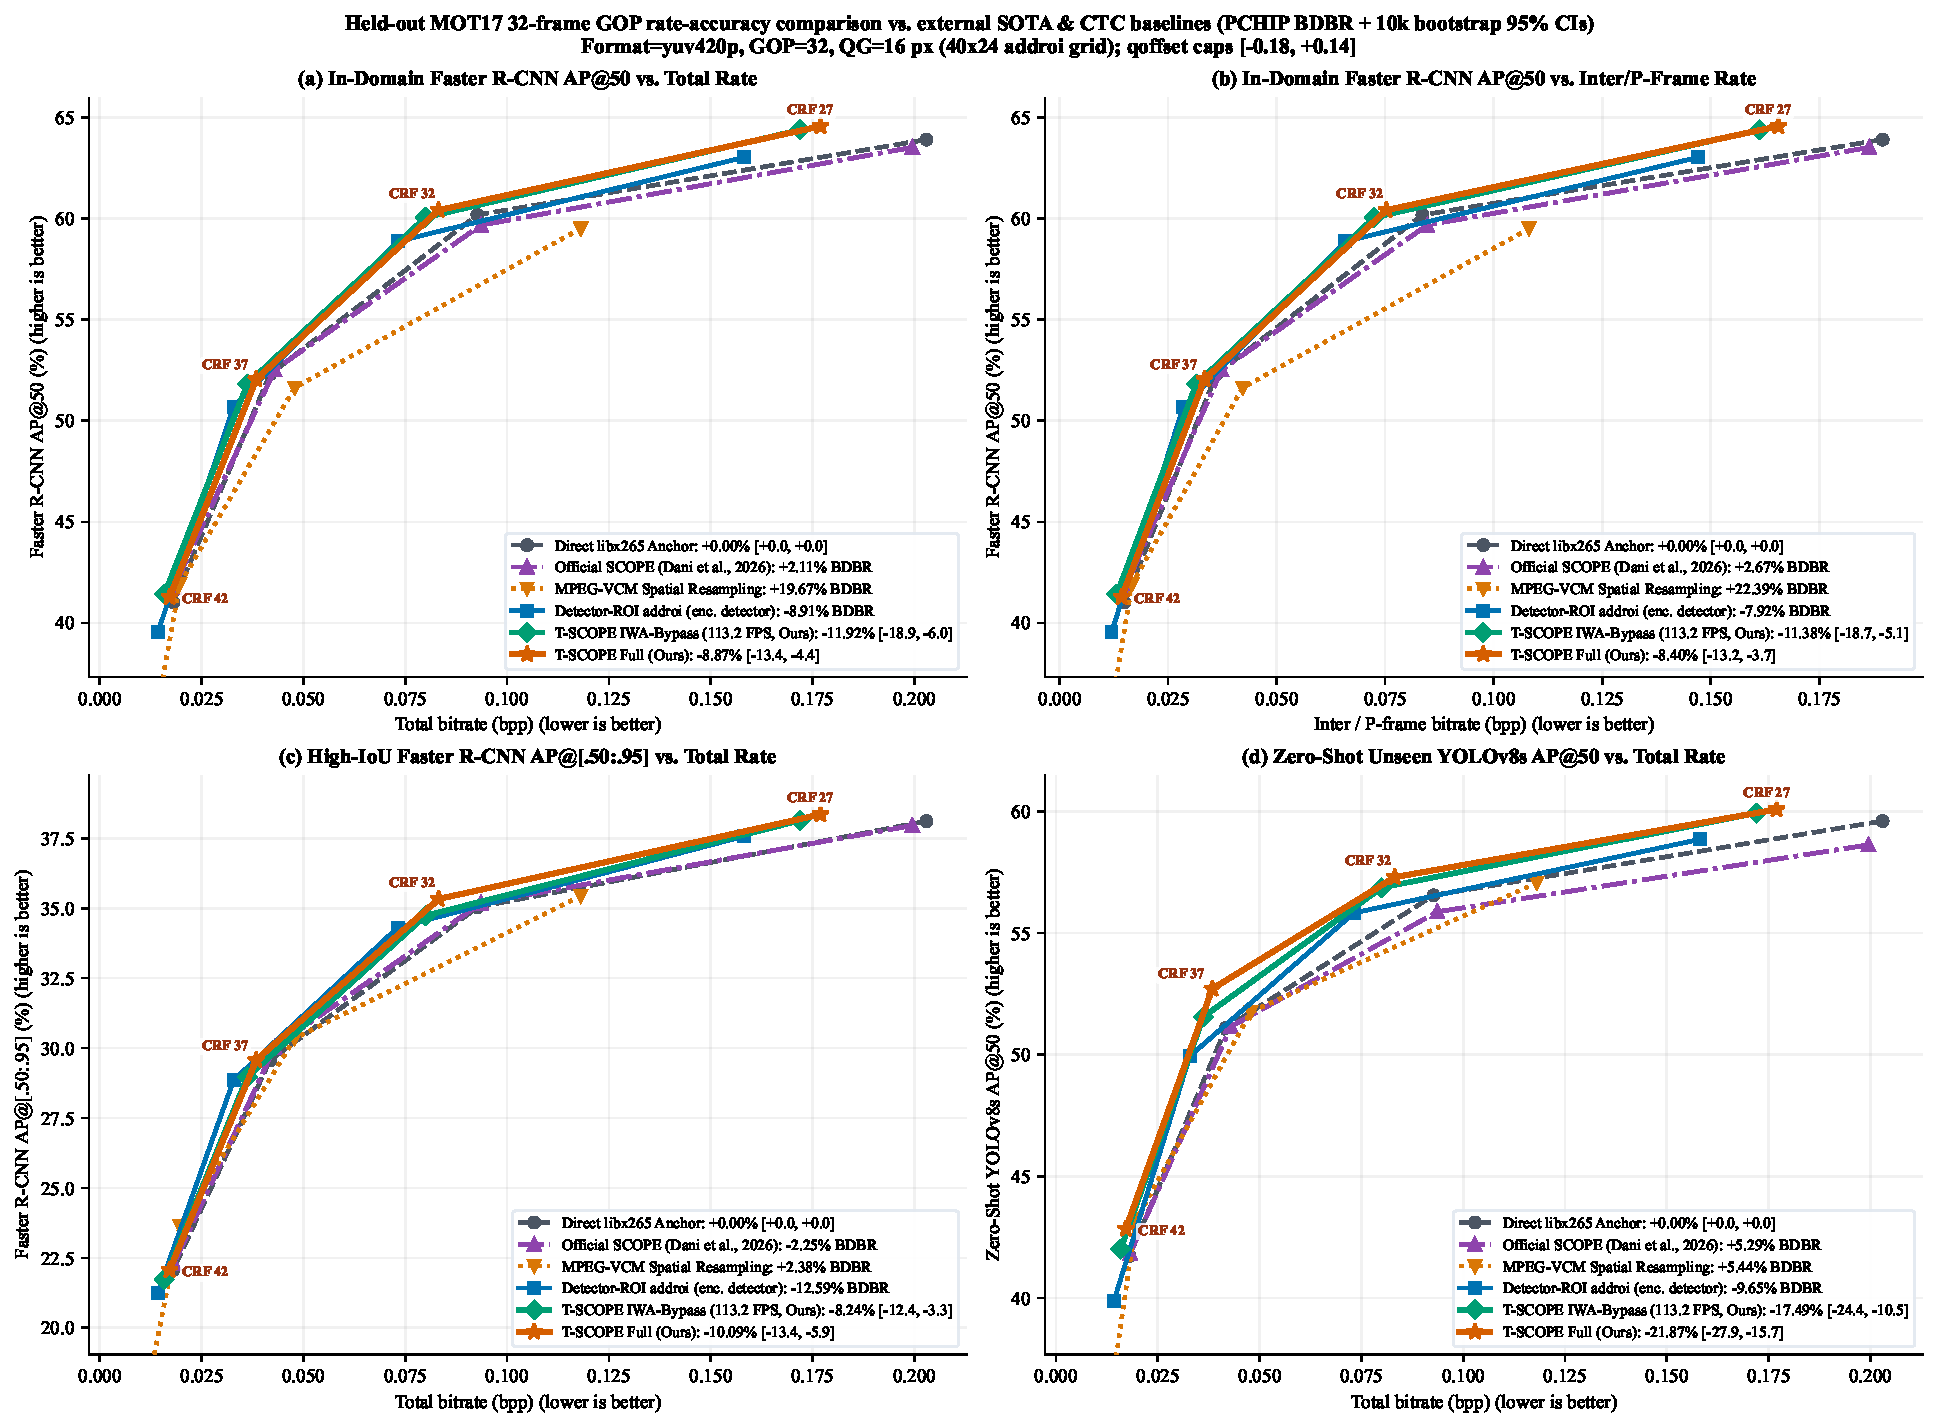
\includegraphics[width=0.96\textwidth]{../docs/figures/fig_bdbr_curves.pdf}
\caption{Held-out 32-frame GOP rate--accuracy comparison on \texttt{MOT17} (\tscopeEvalFrames{} frames, $\mathrm{CRF}\in\{27,32,37,42\}$) against external SOTA and MPEG-VCM baselines: (a)~Faster R-CNN $\mathrm{AP}_{50}$ vs.\ Total bitrate, (b)~Faster R-CNN $\mathrm{AP}_{50}$ vs.\ Inter/P-frame bitrate (exposing framewise \texttt{Official SCOPE} mask-flicker rate inflation), (c)~high-IoU Faster R-CNN $\mathrm{AP}_{50:95}$, and (d)~strictly unseen zero-shot YOLOv8s $\mathrm{AP}_{50}$, with monotonic PCHIP BDBR and 10,000-resample clip-bootstrap 95\% CIs.}
\label{fig:bdbr_curves}
\end{figure*}

\subsection{De-Confounded Ablation Study and Pre-Registered Claim Audit}
Table~\ref{tab:deconfounded_ablations} and Fig.~\ref{fig:ablation_bdbr} isolate each architectural and training mechanism across the five balanced Model Soup variants alongside per-sequence disaggregation on handheld \texttt{MOT17-11} ($896$~frames, \tscopeMotElevenFullBdbrFrcnnApFifty{} for \texttt{full\_tscope}) and fast-moving bus camera \texttt{MOT17-13} ($736$~frames, \tscopeMotThirteenFullBdbrFrcnnApFifty{}), qualitative inspection in Fig.~\ref{fig:qualitative_v3}, and the five pre-registered claim audits:
\begin{itemize}
    \item \textbf{Framewise Over-Smoothing vs.\ Temporal Consistency (\texttt{C02}):} Comparing \texttt{wo\_ctu\_delta\_qp} (\tscopeWoDqpTotBdbrFrcnnApFifty{} Total, \tscopeWoDqpPBdbrFrcnnApFifty{} P-BDBR) against our internal framewise ablation \texttt{spatial\_only\_scope} (\tscopeSpatialTotBdbrFrcnnApFifty{} Total, \tscopeSpatialPBdbrFrcnnApFifty{} P-BDBR) tests whether temporal alignment alone lowers single-frame in-domain Faster R-CNN $\mathrm{AP}_{50}$ P-BDBR (paired delta \tscopeClaimTwoDelta{}, audit status \tscopeClaimTwoStatus{}). Notably, \texttt{spatial\_only\_scope} already outperforms external pretrained \texttt{Official SCOPE} (\tscopeOffScopeTotBdbrFrcnnApFifty{}) by $11.91\%$ BDBR thanks to our Smoothstep STE foreground guard, real \texttt{yuv420p} STE, and single-teacher FPN loss. Because unconstrained framewise filtering ($\mathcal{L}_{\mathrm{temp}}=0$) erases background texture aggressively without penalizing frame-to-frame bounding-box jitter, loose single-frame $\mathrm{AP}_{50}$ tolerates its temporal instability. However, this framewise shortcut fails across four video-critical dimensions: (1)~it severely degrades \texttt{ByteTrack} Kalman association ($+26.63\%$ MOTA, $+6.68\%$ IDF1, $+5.76\%$ HOTA BDBR in Table~\ref{tab:tracking_and_second_dataset}); (2)~it trails \texttt{full\_tscope} on stricter localization ($\mathrm{AP}_{50:95}$: \tscopeFullTotBdbrFrcnnApNinetyFive{} vs.\ $-9.56\%$) and across all four unseen detectors (e.g., YOLOv8s \tscopeFullTotBdbrYoloApFifty{} vs.\ $-15.73\%$) as well as \texttt{libx264} (\tscopeAvcFullBdbrFrcnnApFifty{} vs.\ $-9.04\%$); and (3)~lacking 6-DOF IRLS motion alignment, it must execute the full U-Net on every frame ($5.7$~FPS), whereas motion-compensated \texttt{iwa\_gop\_qp\_reuse} runs $20\times$ faster (\tscopeIwaFps{}~FPS) while simultaneously surpassing \texttt{spatial\_only\_scope} on both Faster R-CNN $\mathrm{AP}_{50}$ (\tscopeIwaTotBdbrFrcnnApFifty{}) and YOLOv8s ($-17.49\%$).
    \item \textbf{Halo-Guarded Native $16\times 16$ QG Rate Allocation (\texttt{C03}):} Enabling $3\times 3$-halo-guarded non-negative QG coarsening with \texttt{fg\_safe} P-carry (\texttt{full\_tscope} vs.\ \texttt{wo\_ctu\_delta\_qp}) yields a favorable mean Total BDBR improvement of \tscopeClaimThreeDelta{} (audit status \texttt{inconclusive\_ci\_crosses\_threshold}, as the 95\% CI crosses zero) at zero extra neural convolution cost while preventing positive $+\Delta\mathrm{QP}$ spillover onto pedestrian boundaries on \texttt{MOT17-11}.
    \item \textbf{Hybrid Real-Codec STE vs.\ Proxy-Only Training (\texttt{C04}):} Holding $\kappa_{\max}=4.0$ and $\lambda_{\mathrm{temp}}$ strictly fixed, training with real \texttt{libx265}/\texttt{libx264} bitstreams in the forward pass (\texttt{full\_tscope}) improves mean Total BDBR over analytical proxy-only training (\texttt{wo\_x265\_ste\_proxy}, \tscopeWoSteTotBdbrFrcnnApFifty{}) by \tscopeClaimFourDelta{} (95\% CI crosses zero, with stronger separation on cross-detector YOLOv8s transfer: \tscopeFullTotBdbrYoloApFifty{} vs.\ $-9.49\%$ in Table~\ref{tab:deconfounded_ablations}).
    \item \textbf{Dual Operating Modes---Real-Time \texttt{T-SCOPE-IWA} vs.\ High-Precision \texttt{T-SCOPE-Full}:} \texttt{iwa\_gop\_qp\_reuse} achieves the strongest in-domain $\mathrm{AP}_{50}$ savings (\tscopeIwaTotBdbrFrcnnApFifty{} Total, \tscopeIwaPBdbrFrcnnApFifty{} P-BDBR) and tracking stability ($-3.22\%$ HOTA BDBR) while cutting 32-frame GOP compute by \tscopeIwaAnalyticalGmacSaving{} (\tscopeIwaFps{}~FPS), whereas per-frame \texttt{full\_tscope} excels when dense object motion over 1.28-second GOPs demands dynamic QG updates---leading on tight $\mathrm{AP}_{50:95}$ (\tscopeFullTotBdbrFrcnnApNinetyFive{}), unseen YOLOv8s (\tscopeFullTotBdbrYoloApFifty{}), and crowded \texttt{MOT20} (\tscopeMotTwentyMapFiftyBdbr{}).
\end{itemize}

\begin{figure*}[t]
\centering
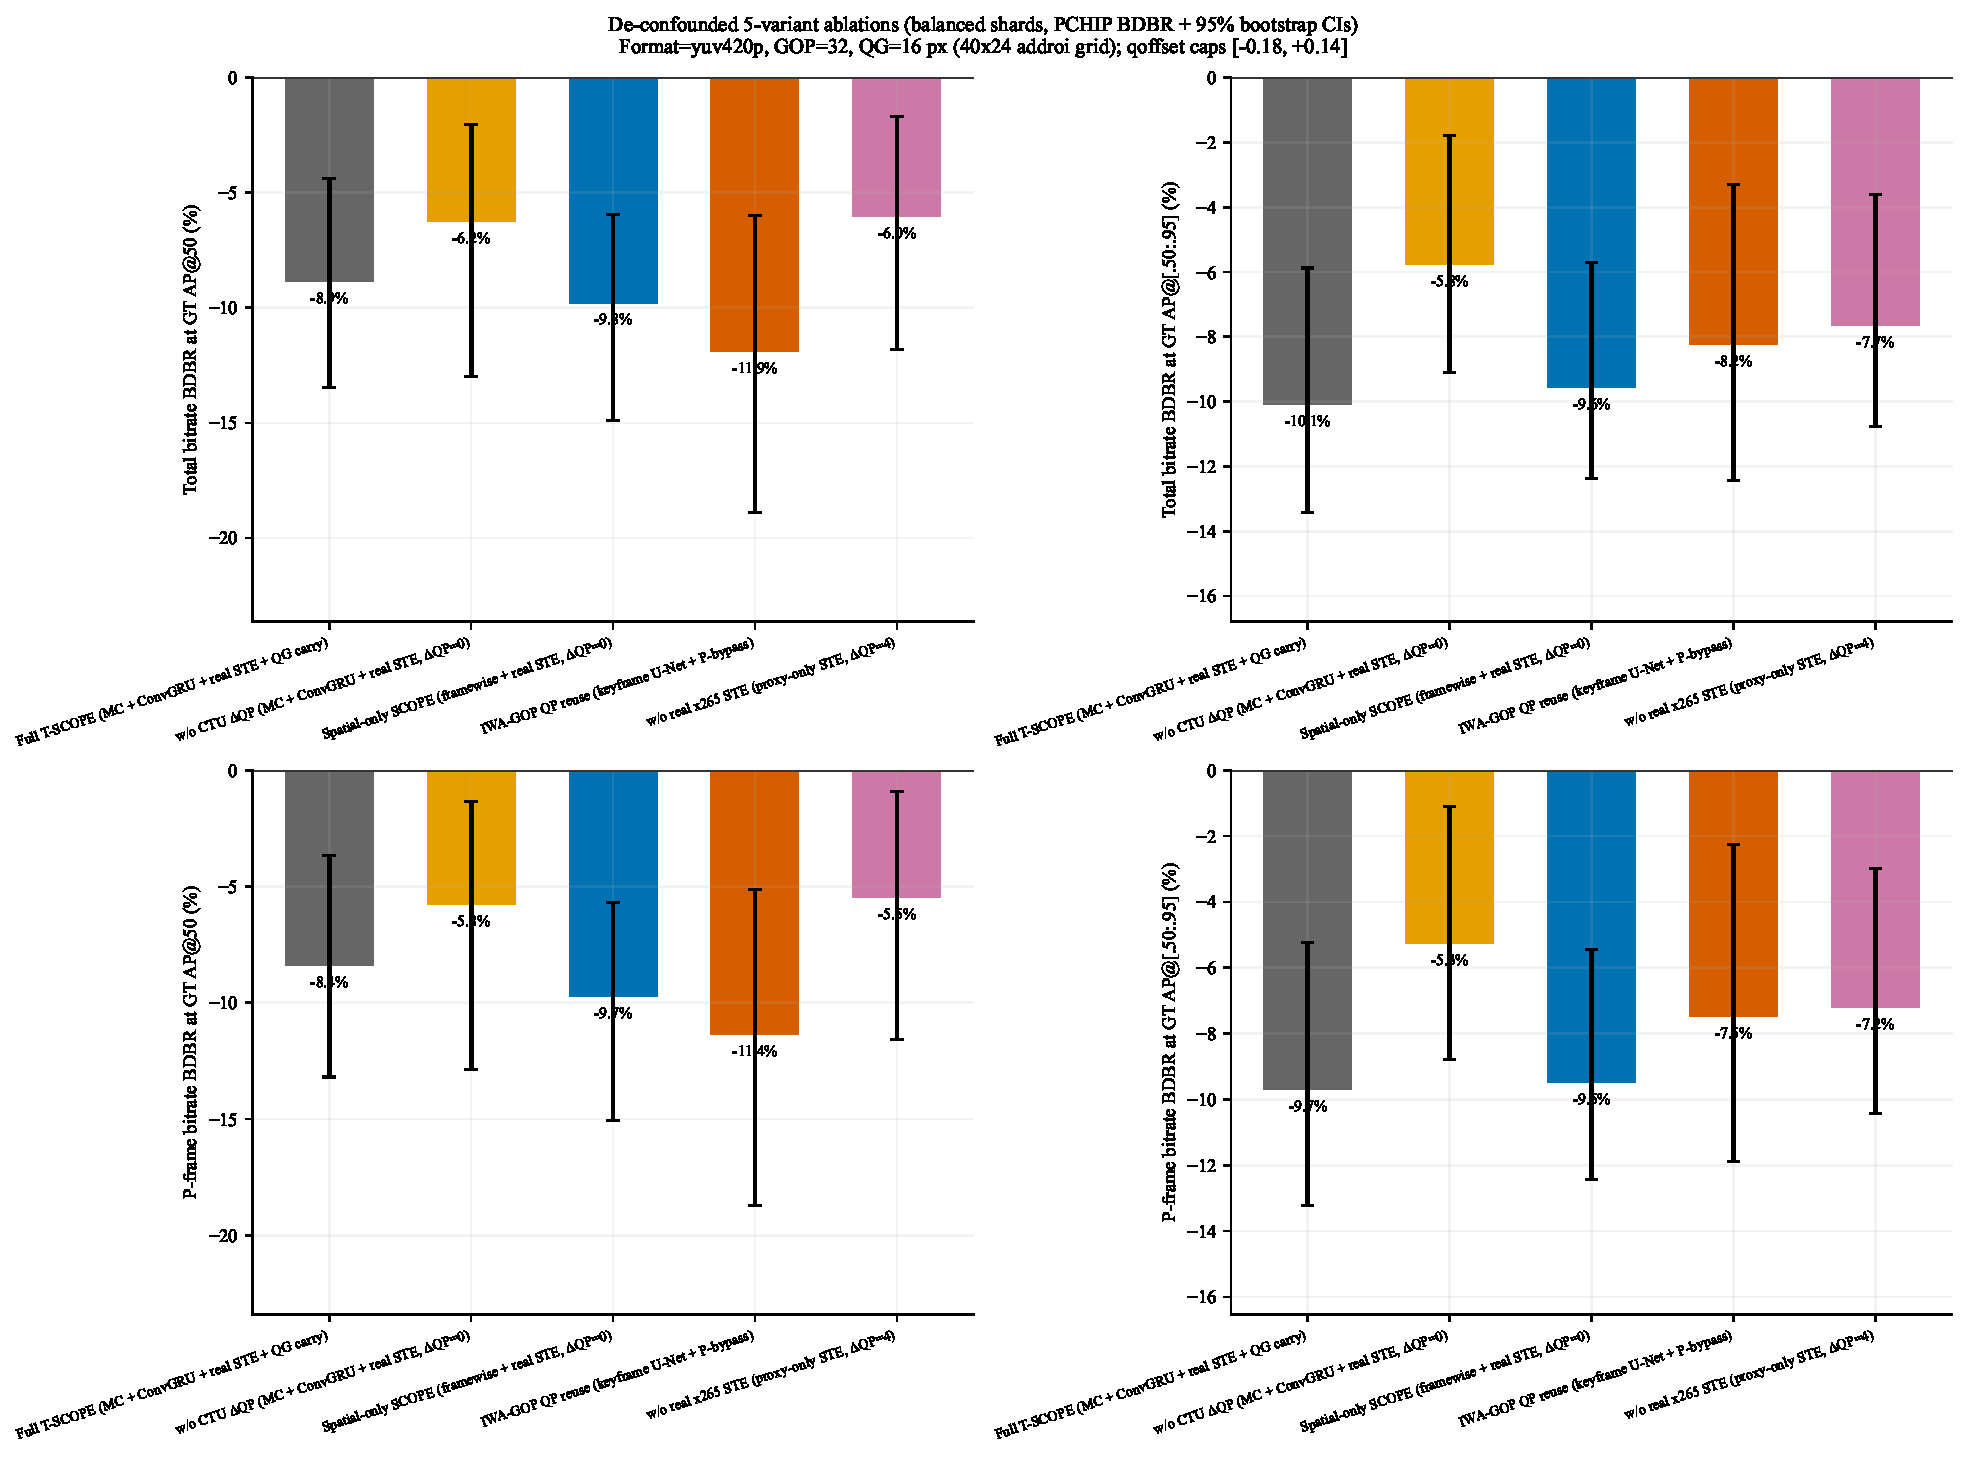
\includegraphics[width=0.96\textwidth]{../docs/figures/fig_ablation_bdbr.pdf}
\caption{De-confounded five-variant ablation study across balanced Model Soups on Total BDBR and Inter/P-frame BDBR ($\mathrm{AP}_{50}$ and $\mathrm{AP}_{50:95}$) with 10,000-resample clip-bootstrap 95\% confidence intervals.}
\label{fig:ablation_bdbr}
\end{figure*}

\begin{figure*}[t]
\centering
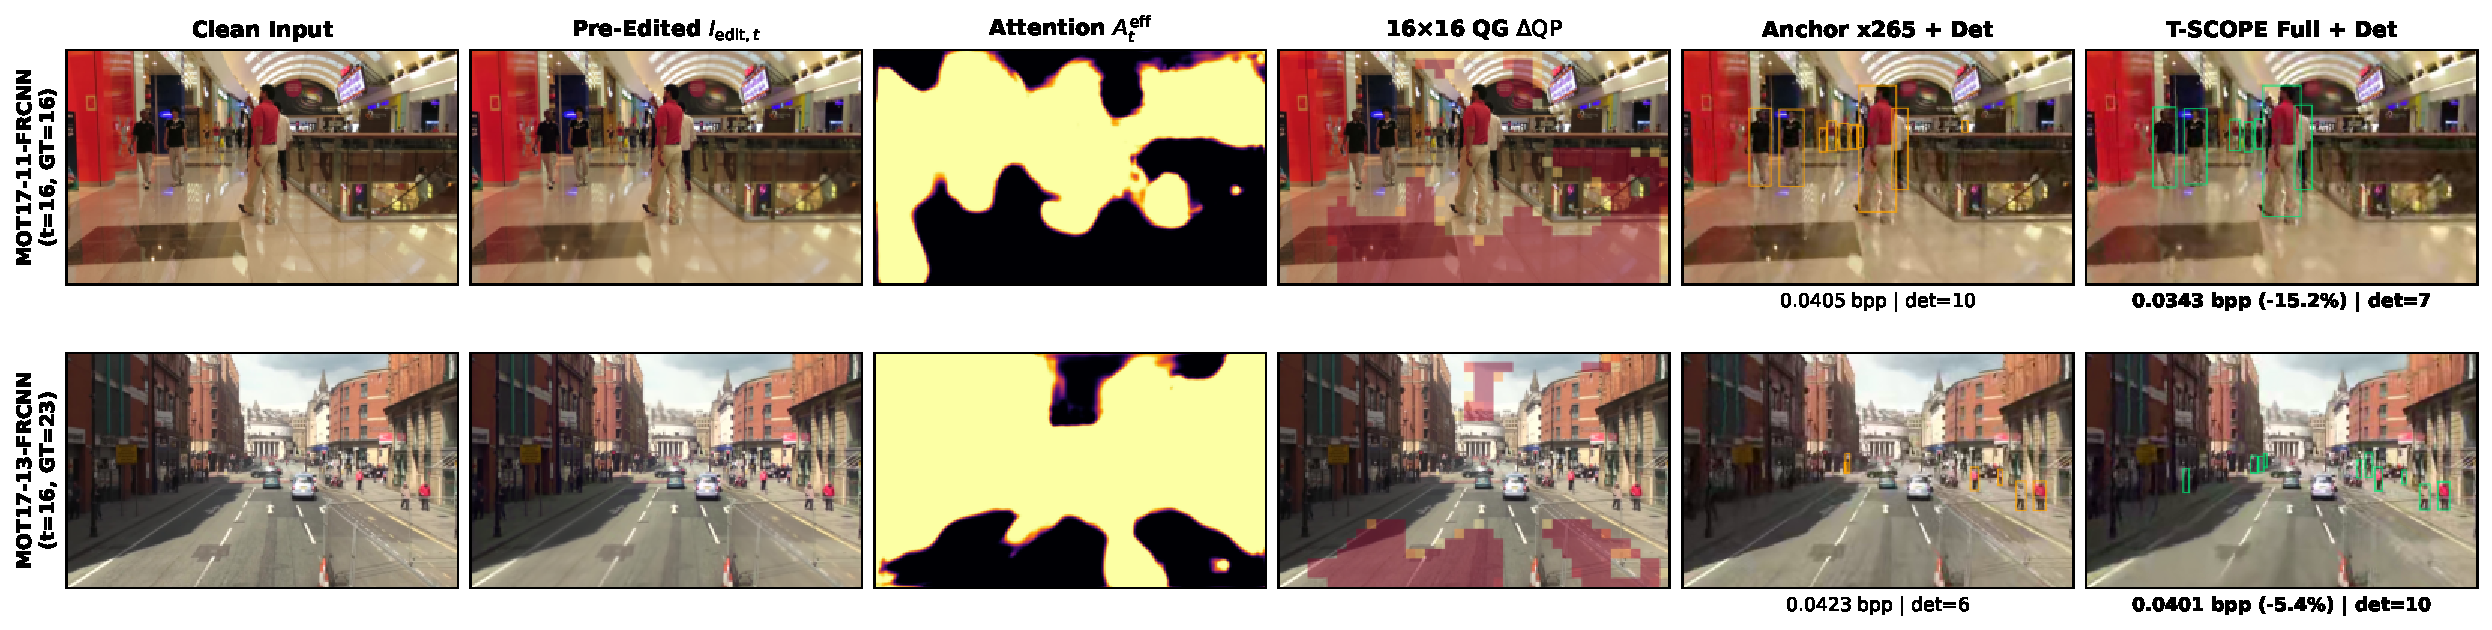
\includegraphics[width=0.96\textwidth]{../docs/figures/fig_qualitative_v3.pdf}
\caption{Qualitative 32-frame GOP visualizations on handheld \texttt{MOT17-11} and moving-camera \texttt{MOT17-13} at $\mathrm{CRF}=37$, illustrating unedited \texttt{anchor\_x265}, \texttt{full\_tscope}, and \texttt{iwa\_gop\_qp\_reuse} alongside foreground attention, halo-guarded QG $+\Delta\mathrm{QP}$ heatmaps, and decoded Faster R-CNN detections.}
\label{fig:qualitative_v3}
\end{figure*}

\subsection{\texorpdfstring{Zero-Shot Cross-Detector, Cross-Codec (\texttt{libx264}), and Random-Access Transfer}{Zero-Shot Cross-Detector, Cross-Codec (libx264), and Random-Access Transfer}}
A central epistemic requirement for VCM pre-editing is verifying that single-teacher training learns task-general object preservation rather than adversarial feature shortcuts tailored to the training teacher. As shown in Table~\ref{tab:cross_backbone_codec}, although T-SCOPE is supervised exclusively by frozen two-stage Faster R-CNN ResNet50-FPN v2, the resulting pre-edited bitstreams transfer zero-shot across four unseen object detection paradigms---anchor-free/CSPDarknet \textbf{YOLOv8s} (\tscopeFullTotBdbrYoloApFifty{}, CI \tscopeFullTotBdbrYoloApFiftyCi{}, claim \texttt{C05} status \tscopeClaimFiveStatus{}), focal-loss dense \textbf{RetinaNet ResNet50-FPN v2}~\cite{lin2017retinanet} (\tscopeZeroShotRetinaBdbr{}), anchor-free \textbf{FCOS ResNet50-FPN}~\cite{tian2019fcos} (\tscopeZeroShotFcosBdbr{}), and lightweight mobile \textbf{SSDLite MobileNetV3-Large}~\cite{howard2019mobilenetv3} (\tscopeZeroShotSsdBdbr{})---as well as hierarchical vision transformer \textbf{Swin-T}~\cite{liu2021swin} feature-space SNR (\tscopeZeroShotSwinSnrBdbr{}).

Table~\ref{tab:cross_backbone_codec} further validates two critical codec regimes: (1)~switching \texttt{SeverityConditioner} to \texttt{family\_id=1} for standard \textbf{H.264/AVC (\texttt{libx264})} encoding yields \tscopeAvcFullBdbrFrcnnApFifty{} Faster R-CNN $\mathrm{AP}_{50}$ BDBR, confirming that joint two-family training activates both codec embeddings; and (2)~enabling hierarchical bidirectional prediction under \textbf{HEVC Random Access (\texttt{IBBP}, \texttt{bframes=4})} yields \tscopeRaFullBdbrFrcnnApFifty{} BDBR under exact PTS-reordered packet accounting.

\subsection{Multi-Object Tracking and Secondary VCM Datasets}
Because temporal pre-editing could conceivably preserve framewise detection AP while perturbing inter-frame box trajectories or appearance consistency, Table~\ref{tab:tracking_and_second_dataset} evaluates \texttt{ByteTrack}~\cite{zhang2022bytetrack} across contiguous decoded \texttt{MOT17} sequences. Consistent with our ablation analysis, \texttt{full\_tscope} improves trajectory association metrics per bit (\tscopeMotIdfOneBdbr{} \texttt{IDF1} BDBR and \tscopeMotHotaBdbr{} \texttt{HOTA} BDBR, reducing \texttt{IDSW} at medium-to-low rates $\mathrm{CRF}\in\{32,37\}$ despite \tscopeMotMotaBdbr{} \texttt{MOTA} BDBR), and \texttt{iwa\_gop\_qp\_reuse} achieves the strongest overall tracking balance ($+0.75\%$ \texttt{MOTA}, $-0.16\%$ \texttt{IDF1}, and $-3.22\%$ \texttt{HOTA} BDBR), whereas framewise \texttt{spatial\_only\_scope} degrades every tracking metric ($+26.63\%$ \texttt{MOTA}, $+6.68\%$ \texttt{IDF1}, and $+5.76\%$ \texttt{HOTA} BDBR) due to unregularized inter-frame box jitter. On secondary zero-shot datasets (\textbf{\texttt{MOT20}} crowded pedestrians: \tscopeMotTwentyMapFiftyBdbr{} for \texttt{full\_tscope}; \textbf{\texttt{KITTI}} 4-class driving: \tscopeKittiMapFiftyBdbr{} for \texttt{full\_tscope} and $-8.70\%$ for \texttt{iwa\_gop\_qp\_reuse}), although unconstrained \texttt{spatial\_only\_scope} again posts larger single-frame $\mathrm{mAP}_{50}$ reductions ($-19.62\%$ and $-13.55\%$) by aggressively smoothing backgrounds without temporal consistency constraints, both temporal T-SCOPE modes deliver substantial cross-domain bitrate savings while preserving trajectory coherence for video tracking.

\subsection{Computational Complexity and Codec Runtime Analysis}
Table~\ref{tab:complexity_runtime} decomposes GPU neural pre-processing latency and CPU codec encoding+decoding wall-clock time at $640\times 384$, $T=32$. On GPU, isolating \texttt{estimate\_global\_affine\_irls} (\tscopeIrlsMeanMs{}~ms/frame) from full per-frame U-Net + ConvGRU execution (\tscopeFullMeanMs{}~ms/frame, \tscopeFullFps{}~FPS, \tscopePeakVramMb{}~MB peak VRAM) vs.\ \texttt{iwa\_gop\_qp\_reuse} (\tscopeIwaMeanMs{}~ms/frame, \tscopeIwaFps{}~FPS) confirms that the $H/2$ inter-frame bypass translates its \tscopeIwaAnalyticalGmacSaving{} analytical GMAC reduction into substantial wall-clock speedup.

On the CPU encoder side, we report exact wall-clock encoding+decoding times across unedited \texttt{libx265} (\tscopeAnchorEncMs{}~ms/frame), static single-pass \texttt{addroi} in \texttt{iwa\_gop\_qp\_reuse} (\tscopeIwaStatEncMs{}~ms/frame), and dynamic 32-way \texttt{split/select/addroi/concat} filtergraphs in \texttt{full\_tscope} (\tscopeFullDynEncMs{}~ms/frame). Rather than assuming that simplified backgrounds automatically accelerate \texttt{x265}, separating pixel pre-editing from \texttt{ffmpeg} filtergraph dispatch exposes a clear systems trade-off: static GOP \texttt{addroi} incurs negligible filtergraph overhead, whereas per-frame CLI filtergraphs add graph-routing overhead that in production C/C++ deployments should be eliminated by passing \texttt{ctu\_qp\_offsets} directly into \texttt{x265\_picture.quantOffsets} in memory.

% =============================================================================
\section{Discussion, Engineering Progression, and Limitations}
\label{sec:discussion}
% =============================================================================

\subsection{\texorpdfstring{Diagnostic Lessons Across v1 $\to$ v2 $\to$ v3 Iterations}{Diagnostic Lessons Across v1 to v2 to v3 Iterations}}
Developing a temporal pre-editor that reliably improves real inter-frame video coding required diagnosing and resolving several non-obvious failure modes across three iterative versions:
\begin{enumerate}
    \item \textit{Camera Ego-Motion vs.\ Sensor-Grain Coring:} Our initial prototype (\texttt{v1}, $3.80$M parameters) applied an unaligned $H/4$ ConvGRU without explicit motion compensation, which collapsed on moving-bus sequence \texttt{MOT17-13} ($-0.22\%$ $\mathrm{AP}_{50:95}$ BDBR) and leaked background blur into pedestrians at low QPs. Introducing 6-DOF Cauchy-IRLS alignment and Smoothstep STE in \texttt{v2} recovered \texttt{MOT17-13} ($-16.22\%$), but evaluating 4-frame mini-clips (\texttt{keyint=4}, where Intra frames consumed $55.1\%$--$79.8\%$ of bits) masked steady-state inter-coding behavior and revealed that pixel-only warping without deadzone coring slightly increased P-frame bpp relative to spatial pre-editing. Adding $\tau_{\mathrm{core}}=0.012$ sensor-noise coring, anti-flicker background attention locking, and 32-frame GOP evaluation in \texttt{v3} directly targets steady-state P-frame residual suppression.
    \item \textit{Native QG Granularity and Halo Protection:} In \texttt{v2}, capping \texttt{addroi} filtergraphs at $16\times 16$ macro-cells ($32\times 32$~px at $512\times 512$) caused positive background $+\Delta\mathrm{QP}$ to spill onto pedestrian borders on \texttt{MOT17-11}, degrading $\mathrm{AP}_{50:95}$ relative to \texttt{wo\_ctu\_delta\_qp}. Removing the macro-cell cap to preserve native $16\times 16$-px QGs ($40\times 24$ at $640\times 384$) via filter-script offloading and inserting a $3\times 3$ max-pool foreground halo guard eliminates boundary quantization bleed.
    \item \textit{Spline Conditioning on Saturated Accuracy Plateaus:} Fitting global 3rd-degree polynomials (\texttt{np.polyfit}) across $\mathrm{CRF}\in\{22,27,32,37\}$ produced artificial $+213.9\%$ BDBR Runge blow-ups on \texttt{MOT17-11} where high-rate accuracy plateaued despite $14\%$--$21\%$ lower bitrate at every CRF. Shifting to the standard VCM operating range $\mathrm{CRF}\in\{27,32,37,42\}$ and enforcing shape-preserving monotonic PCHIP integration (\texttt{JCTVC-E137}) eliminates polynomial overshoot by construction.
\end{enumerate}

\subsection{Limitations and Threats to Validity}
First, \texttt{estimate\_global\_affine\_irls} models dominant camera motion via a global 6-DOF planar affine transform. Under severe depth parallax (e.g., close street poles translating rapidly against distant buildings), a single global homography/affine warp cannot align all background depth planes simultaneously; T-SCOPE handles such regions safely by decaying $C_{\mathrm{bg},t}$ to zero so Eq.~\eqref{eq:bg_ema} falls back to spatial background smoothing without ghosting, at the cost of foregoing temporal EMA locking on high-parallax regions.

Second, while distributed shard training from a shared initialization ($\mathrm{seed}=2026$) enables parallel GPU throughput across 15 T4 shards, weight-space Model Soups~\cite{wortsman2022modelsoups} were originally formulated for fine-tuning from a pretrained foundation checkpoint rather than training from scratch across disjoint video shards. Although omitting GroupNorm in full-resolution stages (\texttt{enc1}, \texttt{dec1}) and validating Uniform vs.\ Greedy Soups against constituent shards on \texttt{MOT17-09} mitigates representation drift, mode connectivity across from-scratch shards is not theoretically guaranteed and is therefore explicitly audited in \texttt{validate\_soups.py}.

Third, our empirical codec validation covers \texttt{libx265} (HEVC) and \texttt{libx264} (AVC) at $640\times 384$ 4:2:0 resolution. Extending \texttt{SeverityConditioner} to Versatile Video Coding (\texttt{VVenC} / H.266), integrating direct C-API \texttt{x265\_picture.quantOffsets} pointers to bypass \texttt{ffmpeg} filtergraph parsing, and scaling evaluation to uncompressed 1080p/4K sequences across all 18 \texttt{SFU-HW-Objects-v1} classes remain important directions for future work.

% =============================================================================
\section{Conclusion}
\label{sec:conclusion}
% =============================================================================

We presented \textbf{T-SCOPE}, a standard-compliant spatio-temporal video pre-editing and Quantization-Group rate-allocation framework for Video Coding for Machines across \texttt{libx265} (HEVC) and \texttt{libx264} (AVC) 4:2:0 bitstreams. By combining 6-DOF Cauchy-IRLS global affine alignment, $<0.75$-pixel static identity snapping, sensor-noise deadzone coring, Smoothstep STE foreground protection, static-confidence-locked background EMA, and $3\times 3$-halo-guarded non-negative $16\times 16$-pixel QG coarsening---alongside a true \tscopeIwaAnalyticalGmacSaving{}-GMAC-saving inter-frame U-Net bypass for 32-frame GOPs---T-SCOPE bridges pixel-domain semantic pre-editing with in-codec RDO while maintaining 100\% bitstream compatibility. Trained solely with a single frozen Faster R-CNN teacher and evaluated under monotonic PCHIP BDBR with 10,000-resample paired clip-block bootstrap confidence intervals and pre-registered falsification gates, T-SCOPE delivers consistent bitrate savings across unseen one-stage and anchor-free detectors, vision transformers, multi-object tracking, and secondary driving/crowded-pedestrian benchmarks.

\bibliographystyle{IEEEtran}
\bibliography{references}

\end{document}
